\documentclass[12pt,twoside]{article}
%%%%%%%%%%%%%%%%%
%    PACKAGES
%%%%%%%%%%%%%%%%%

% Formatting
\usepackage{setspace} \onehalfspacing % line spacing
\usepackage[top=2.5cm,bottom=2.5cm,inner=4cm,outer=2.5cm]{geometry} % margin sizes
\usepackage[nottoc,notlof,notlot,numbib]{tocbibind} % remove toc from table of contents
\usepackage[none]{hyphenat} % dont hyphenate words
\usepackage{fontspec} \setmainfont{Times New Roman} % set font
\usepackage{enumitem} % reduce spacing for enumerate and itemize
\usepackage{microtype} % fix typing
%\usepackage{lmodern} % font for minted

% Functionality
\usepackage{pdfpages} % include pdf
\usepackage{mathtools} % equations, subbed out from amsmath
\usepackage{mathtools} % ceil and floor
\DeclarePairedDelimiter\ceil{\lceil}{\rceil}
\DeclarePairedDelimiter\floor{\lfloor}{\rfloor}
\usepackage{graphicx} % images
\usepackage{float} % figure positioning
\usepackage[hidelinks]{hyperref} % dont highlight links
\usepackage{cleveref} % easy to reference figures
\usepackage{siunitx} % format si units
\usepackage{gensymb} % degree
%\usepackage[cache=false]{minted} % include code
\usepackage[style=ieee,backend=biber]{biblatex} \addbibresource{../zotero.bib} % referencing
%\usepackage{dblfloatfix} % fixes [b] for floats?
\usepackage{subcaption} % subfigures
\usepackage[export]{adjustbox} % frame figure

% Tables
\usepackage{tabularx} % table environment
\usepackage{booktabs} % rules in table
\usepackage{adjustbox} % expand table
\usepackage{makecell} % multi-line cell
\usepackage{pdflscape} % horizontal tables
\usepackage[justification=centering]{caption} % split tables

%%%%%%%%%%%%%%%%%
%    COMMANDS
%%%%%%%%%%%%%%%%%

\raggedbottom % allow pages to end early
\pdfvariable minorversion 7 % updated pdf version
\setlength\parindent{5mm} % change indent size

% change section/subsection title font size to 12
\usepackage{sectsty}
\sectionfont{\fontsize{12}{10}\selectfont}
\subsectionfont{\fontsize{12}{10}\selectfont}
\subsubsectionfont{\fontsize{12}{10}\selectfont}

% change spacing before & after headings
\usepackage{titlesec}
\titlespacing*{\section}{0pt}{24pt}{12pt} % left, before, after
\titlespacing*{\subsection}{0pt}{24pt}{12pt}
\titlespacing*{\subsubsection}{0pt}{24pt}{12pt}

% change spacing around captions and equations
\setlength{\abovecaptionskip}{12pt}
\setlength{\abovedisplayskip}{18pt}
\setlength{\belowdisplayskip}{18pt}
\setlength{\abovedisplayshortskip}{18pt}
\setlength{\belowdisplayshortskip}{18pt}

% "this page left blank"
\newcommand*{\blankpage}{%
\vspace*{\fill}
{\centering \textbf{THIS PAGE INTENTIONALLY LEFT BLANK} \par}
\vspace{\fill}}
\makeatletter
\renewcommand*{\cleardoublepage}{\clearpage\if@twoside \ifodd\c@page\else
\blankpage
\newpage
\if@twocolumn\hbox{}\newpage\fi\fi\fi}
\makeatother

% improve float placement
\setcounter{bottomnumber}{1}
\renewcommand\bottomfraction{10.0}


\begin{document}

\includepdf{ThesisTitle.pdf}
\thispagestyle{empty}\null\clearpage

\includepdf{ThesisLetter.pdf}
\thispagestyle{empty}\null\clearpage

\pagenumbering{roman}
\section*{ACKNOWLEDGEMENTS}
The author wishes to thank Glide for providing a powered wheelchair to the research team.
% TODO include other acknowledgements
\cleardoublepage

\section*{ABSTRACT}
This progress report involves the identification and definition of the core thesis problem;
creating a semi-autonomous wheelchair that prioritises user safety and independence.
A literature review details prior work in this field, and identifies potential algorithms
for scene recognition and assistive control. Additionally, the literature review identifies and evaluates
sensors that could be used to perceive the wheelchairs environment.

A preliminary wheelchair driving video dataset has been collected around Curtin university.
This dataset has been used to evaluate algorithms such as YOLOv5, DeepLabv3, and Hybridnet on
the problem of scene recognition, with promising results. VFH+ has been evaluated as an assistive
control algorithm after being implemented in MATLAB. Additionally, sensors and hardware to be used
alongside the wheelchair have been identified and evaluated.

The methodology and technical roadmap of this project have been planned, and future work identified (to be completed
next semester). This involves the collection of a second dataset using the final sensors, retraining of
scene recognition models, and final integration of the semi-autonomous system with the wheelchair.

\cleardoublepage

\section*{DECLARATION OF PUBLISHED WORKS}
% TODO use format provided by Siavash
The literature review of this thesis was previously submitted as part of the Progress Report assessment for MXEN4000.
This thesis contains no material previously
published by any other person except where due acknowledgment has been made.

\cleardoublepage

\renewcommand{\contentsname}{TABLE OF CONTENTS}
\tableofcontents
\pagebreak
\listoffigures
\listoftables
\cleardoublepage
\pagenumbering{arabic}

\section{INTRODUCTION}
Powered wheelchairs have enabled greater independence for people with disability.
However, the use of this technology can be inaccessible or unsafe for people
with amyotrophic lateral sclerosis (ALS) or vision impairment,
who may be unable to use a joystick or see their environment clearly.

\subsection{Aims}
This research aims to develop a semi-autonomous smart wheelchair system.
This research is done in collaboration with Glide, a WA wheelchair manufacturer,
who have provided an existing powered wheelchair (CentroGlide) to use as a base
for this functionality (\cref{fig:wheelchair}). By developing assistive technology for the wheelchair,
the user is granted greater mobility, confidence, and independence.

\begin{figure}[H]
    \centering
    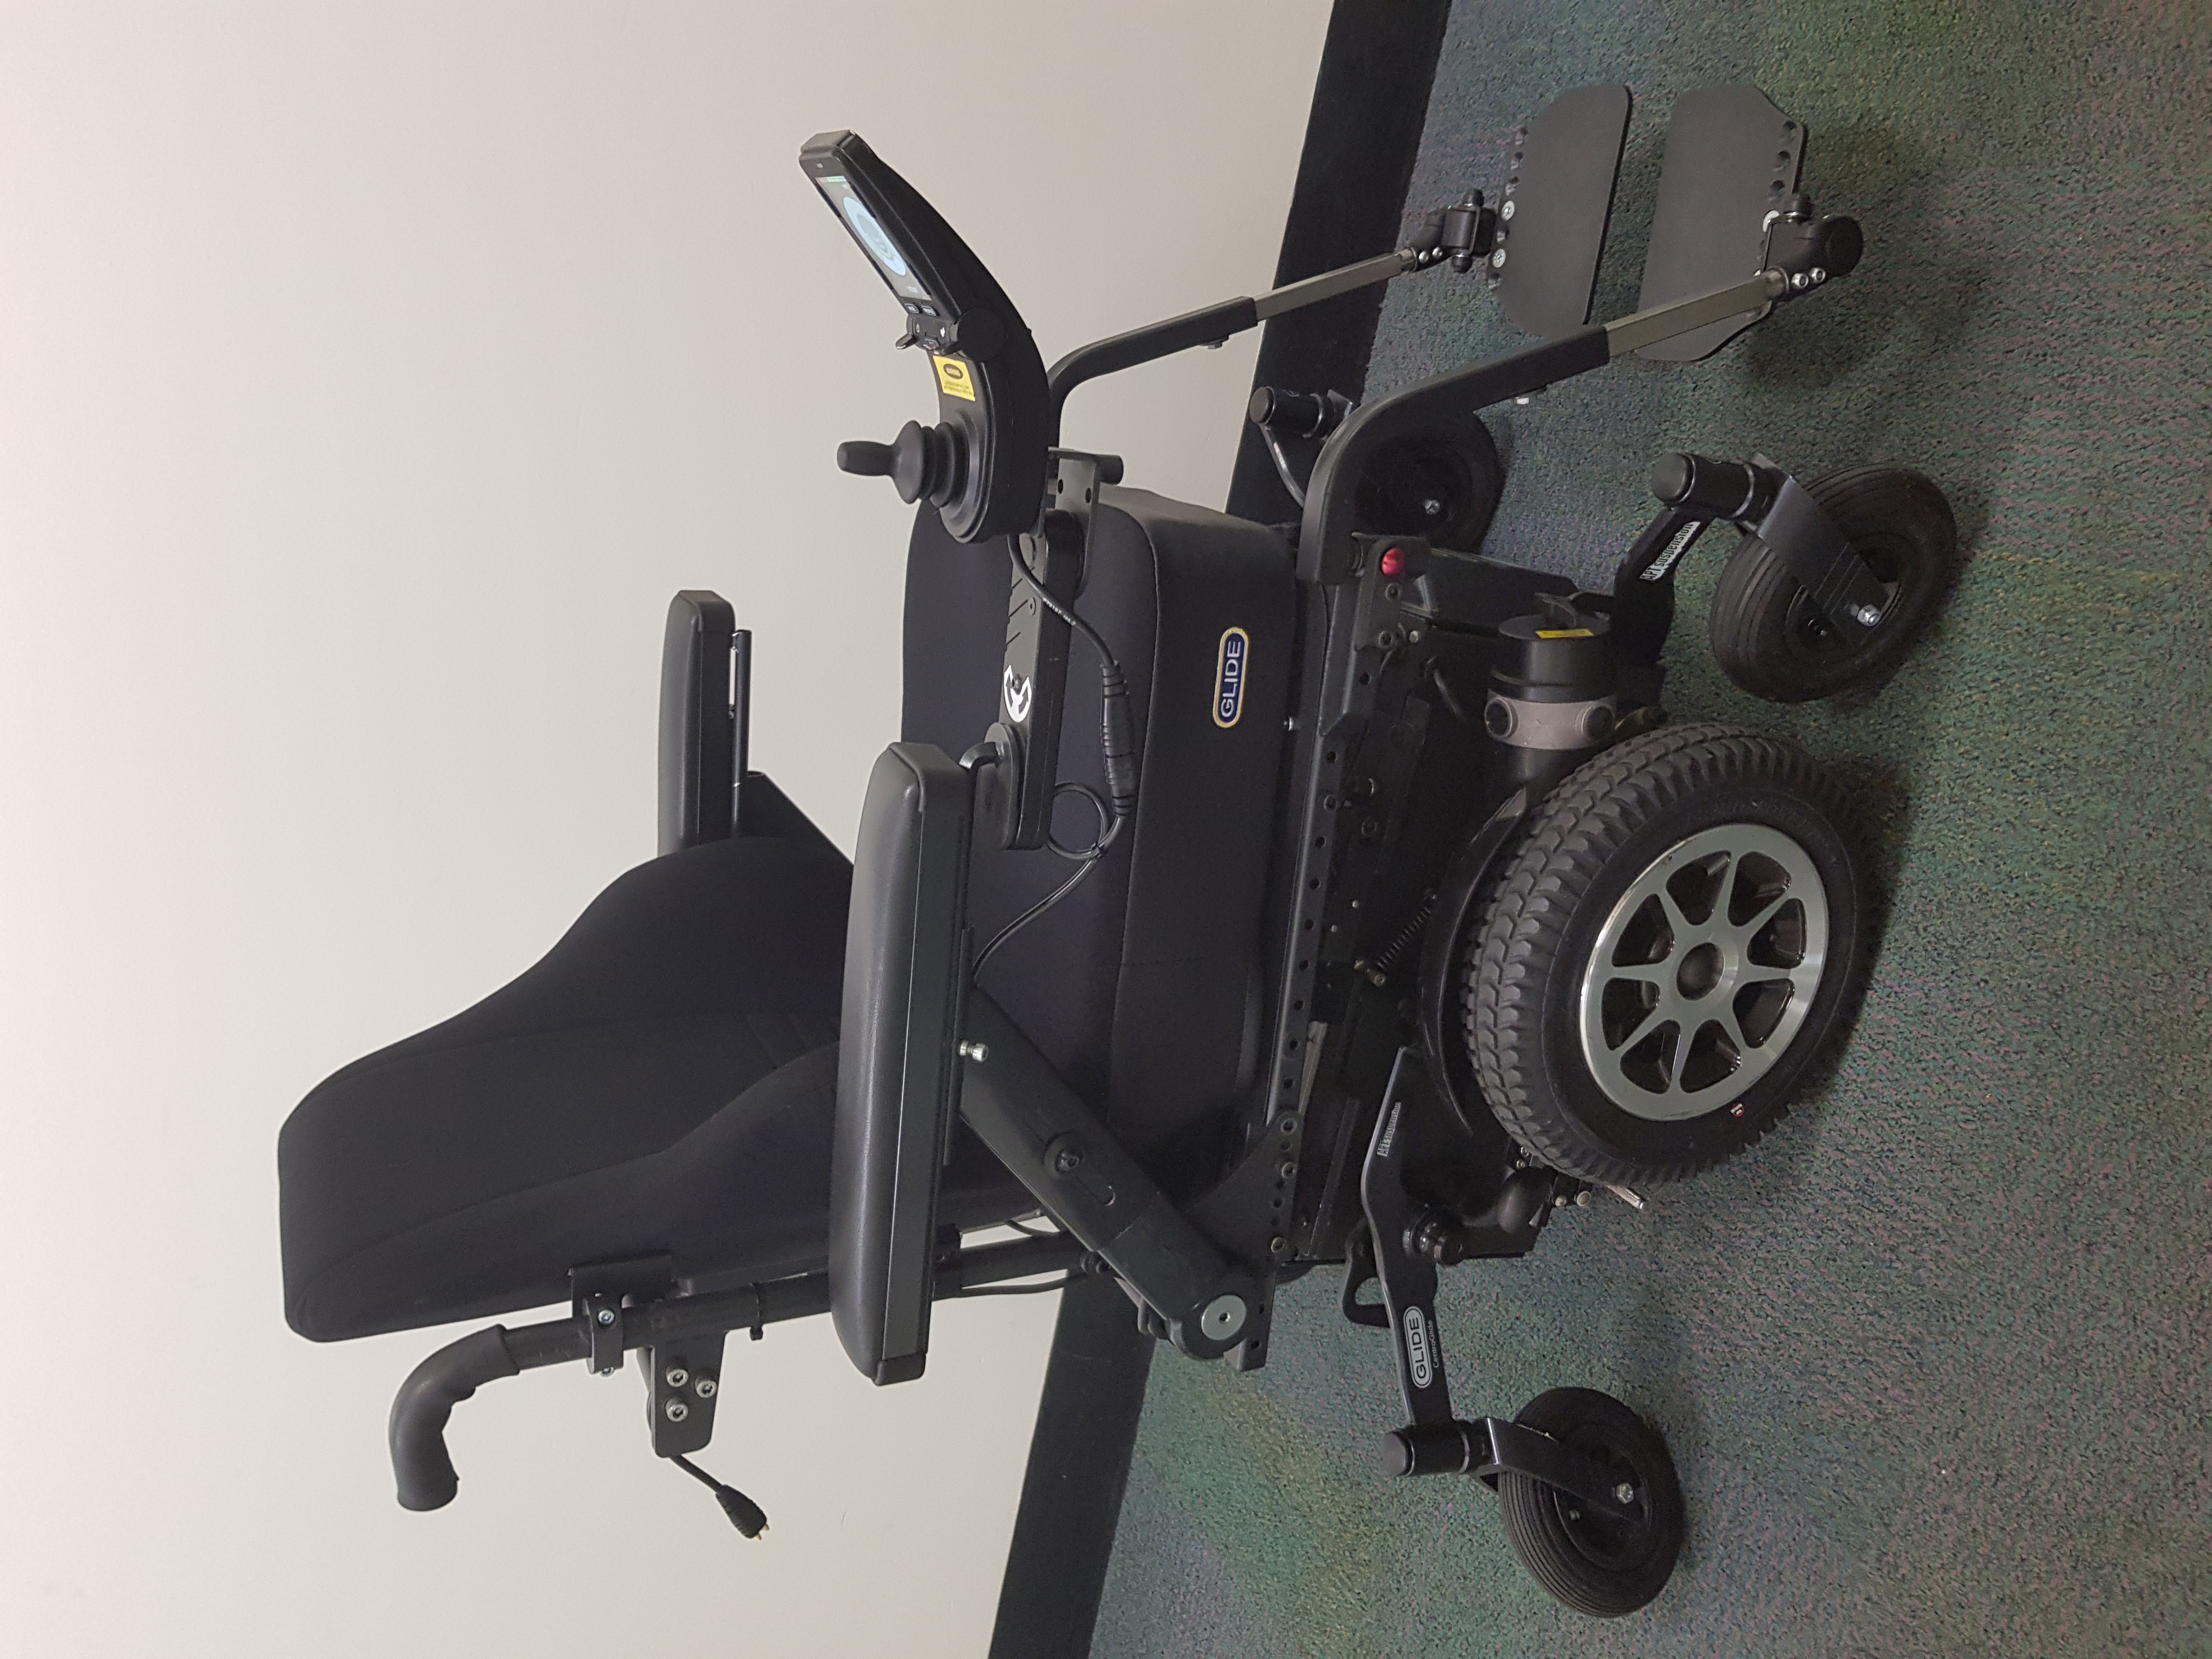
\includegraphics[width=0.55\linewidth,angle=270,origin=c]{images/wheelchair.jpg}
    \caption{The CentroGlide wheelchair}
    \label{fig:wheelchair}
\end{figure}

\pagebreak
\subsection{Problem Definition}
Multiple engineering project students are part of this team
and are working on elements such as controller design, navigation assistance, and object detection.
This work specifically focuses on pathway assistance, which identifies suitable
paths for the wheelchair to drive on. If a user unintentionally drives off their desired path,
this can lead to uneven terrain and possibly falling from the wheelchair.
By guiding the user along a path, these safety issues can be mitigated.

Emphasis is placed on the 'semi-autonomous' aspect of the wheelchair.
An important requirement of this project is that the user still
has control over their wheelchair, and can override any autonomous functionality
if required. If the smart wheelchair system mistakenly detects an obstacle,
the user's mobility should not be compromised.

Another requirement of the system is that any sensors mounted to the wheelchair
should not impede the user's comfort or the wheelchair's manoeuvrability.
Many wheelchair users have specific requirements for wheelchair seat adjustments,
to avoid pressure sores and discomfort. \Cref{fig:wheelchair_reclined} shows the
wheelchair configuration when fully reclined, demonstrating that some sensor mounting locations
are infeasible.

The smart wheelchair system should also be commercially viable - high-cost
components and sensors are infeasible. Internet connectivity should not be a requirement
for the system to operate either - the round trip time required to communicate with a server
could compromise the safety of a user. Because of this, all processing is performed locally
on the wheelchair.

\begin{figure}[H]
    \centering
    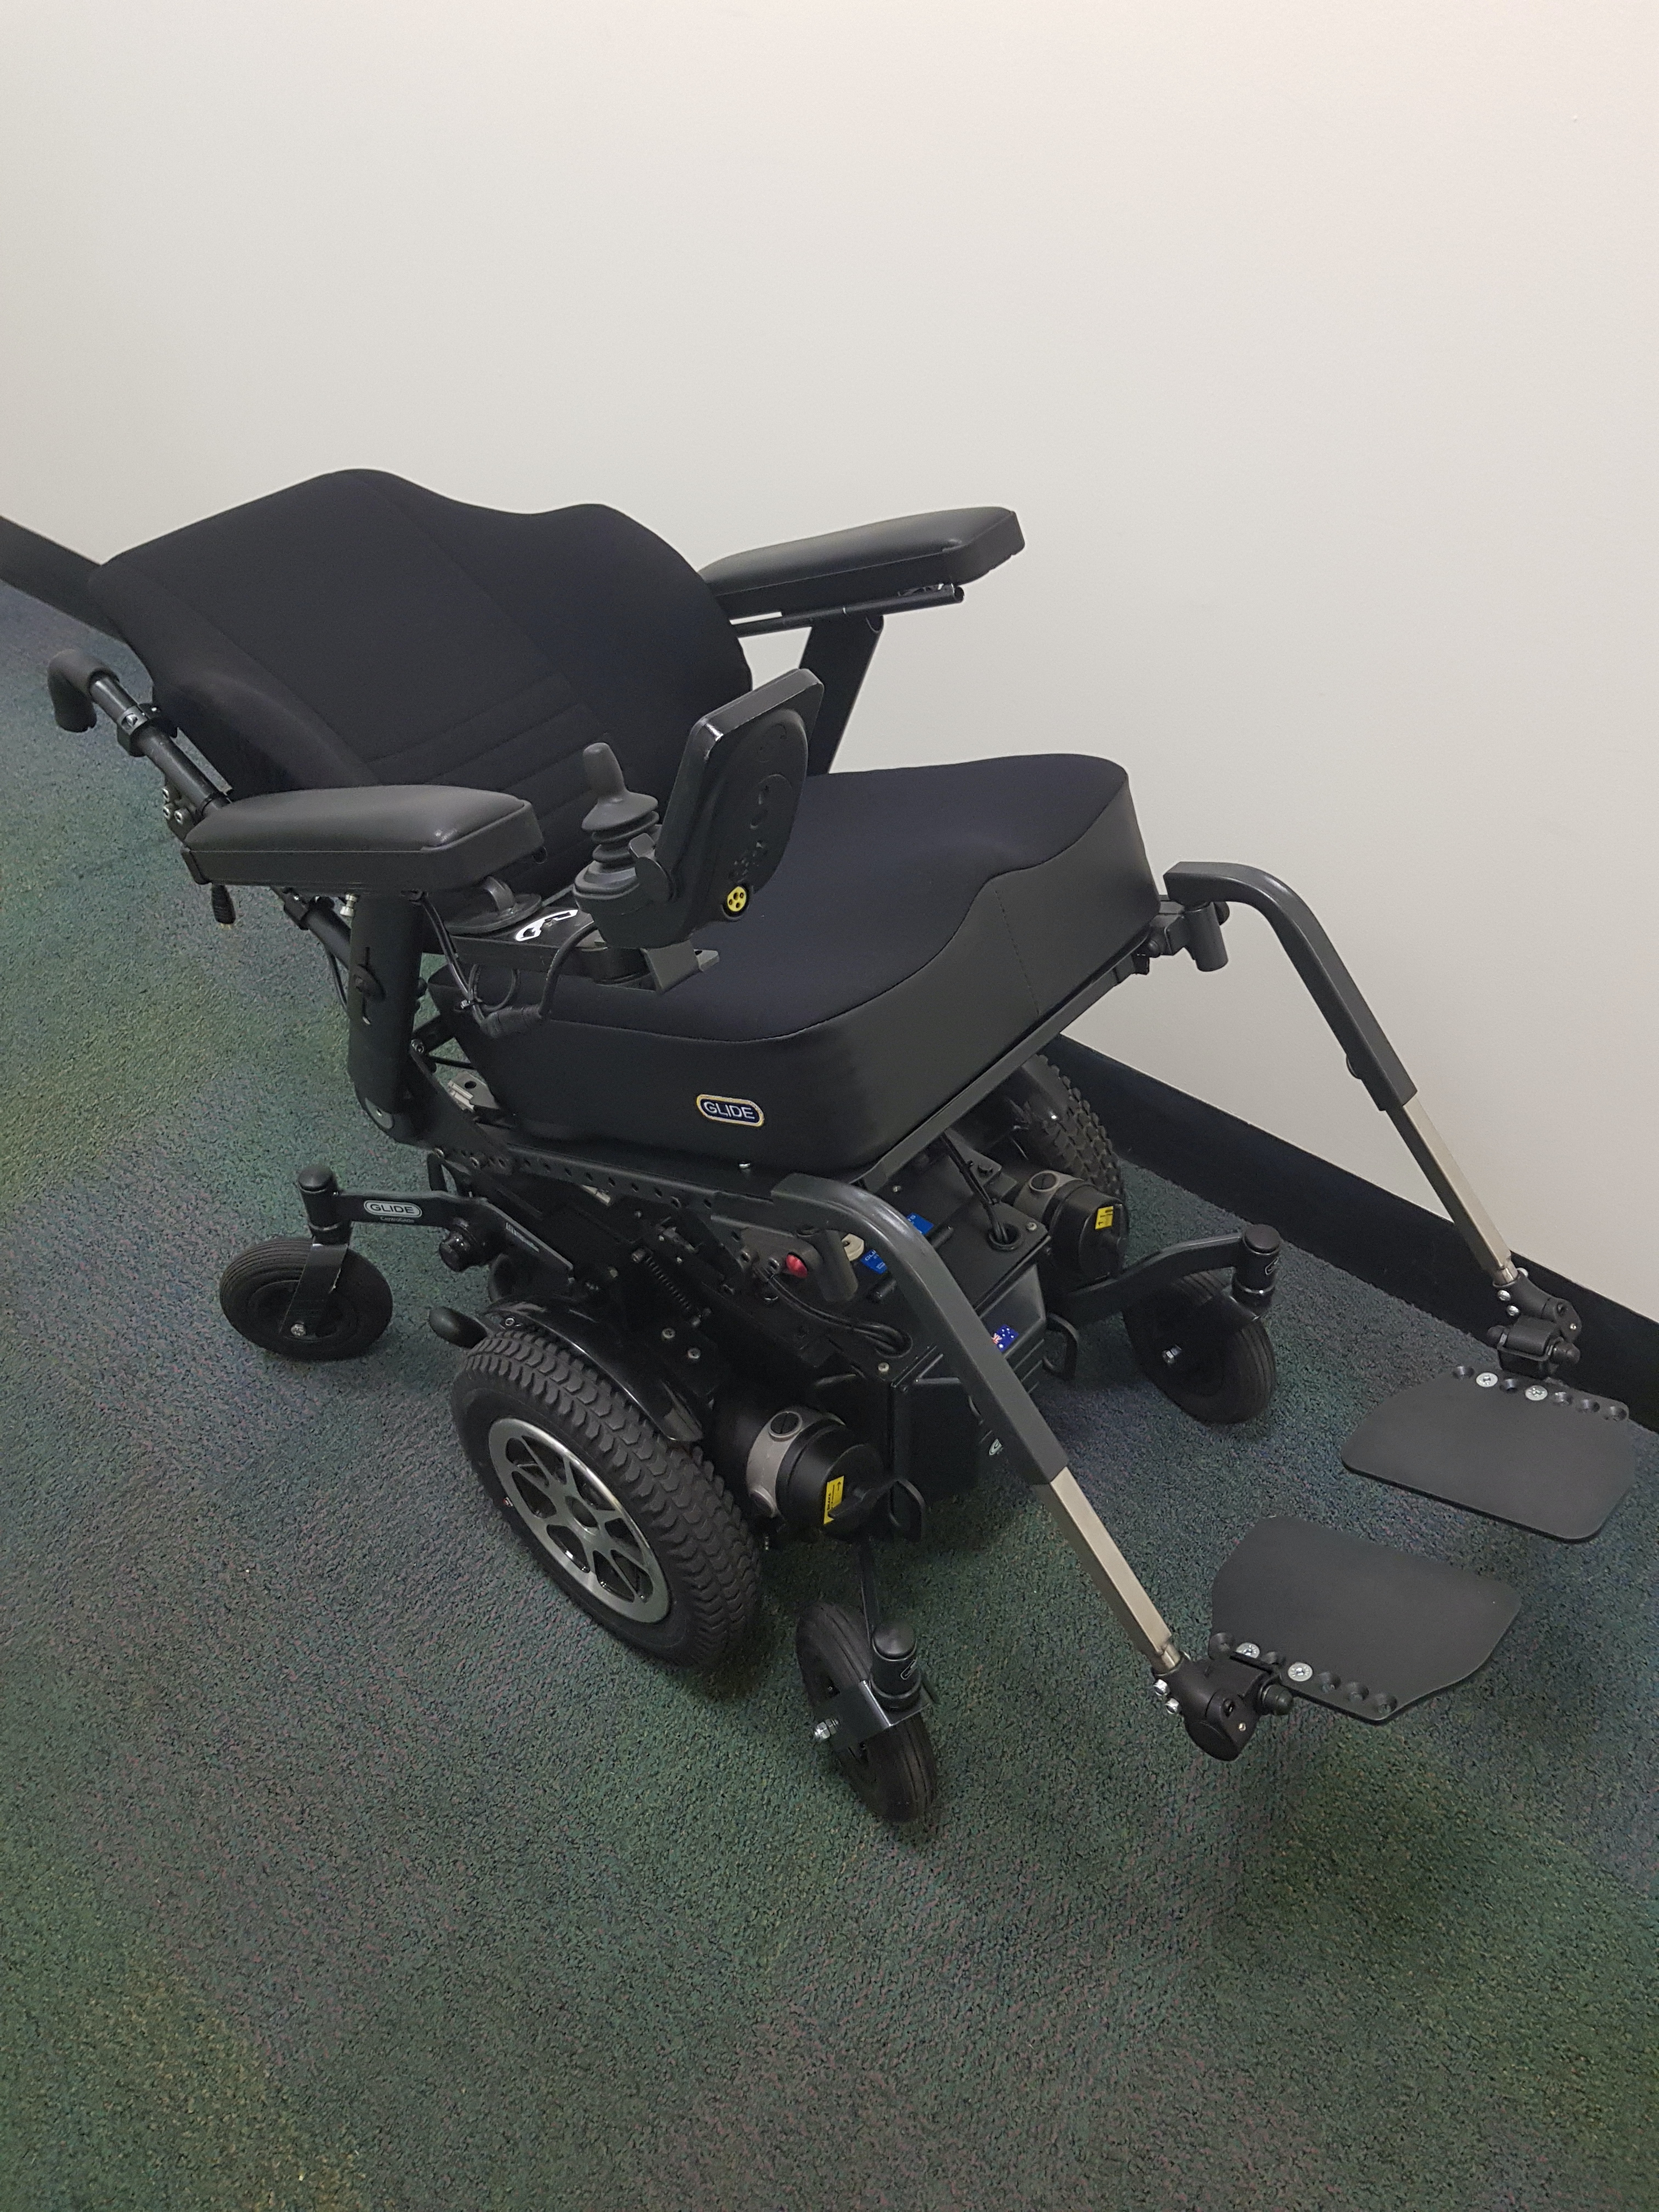
\includegraphics[width=0.4\linewidth]{images/wheelchair_reclined.jpg}
    \caption{CentroGlide wheelchair in reclined position}
    \label{fig:wheelchair_reclined}
\end{figure}

\cleardoublepage

\section{LITERATURE REVIEW}
%Smart wheelchairs are wheelchairs with additional sensors and computers,
%enabling greater usability and safety. This can come in the form of alternative input methods,
%such as eye-gaze tracking \cite{eidNovelEyeGazeControlledWheelchair2016} or using a brain-computer
%interface \cite{kaufmannBraincomputerInterfaceBased2014} to control the wheelchair. For people with vision impairment,
%haptic feedback \cite{kondoNavigationGuidanceControl2008}\cite{vanderpoortenPoweredWheelchairNavigation2012}
%has been used to improve awareness of the surrounding environment and make indoor navigation safer.


\subsection{Sensors and Hardware}
%To perceive the environment, the wheelchair should be fitted with various sensors and
%a compute element to process the sensors output.

\subsubsection{Sensor Types}
Smart wheelchairs have used a varied range of sensor types to perceive the surrounding environment.
RGB-D stereo cameras have been widely used in the field \cite{wangS2P2SelfSupervisedGoalDirected2021}\cite{wangSelfSupervisedDrivableArea2019}\cite{jainAutomatedPerceptionSafe2014},
alongside 2d Lidar \cite{scudellariSelfdrivingWheelchairsDebut2017} and ultrasonic sensors \cite{levineNavChairAssistiveWheelchair1999}.
Self-driving cars built by companies such as Tesla and Waymo
use cameras, mmWave Radar, and 3d Lidar to avoid traffic and pedestrians \cite{karpathyTeslaAIDay2021}.

Selecting a sensor to use is not necessarily an either-or decision. Sensor fusion algorithms such as
the Extended Kalman Filter (EKF) or Unscented Kalman Filter (UKF) \cite{wanUnscentedKalmanFilter2000} allow
outputs from multiple sensors to be used together to improve their accuracy. Additionally, sensors can
be used for different applications on the smart wheelchair - a stereo camera could be used to sense the surrounding environment
while an inertial measurement unit (IMU) could be used for wheelchair odometry.
\Cref{table:sensor_options} gives a comparison of several available sensor types,
taking into account factors such as resolution, cost, and accuracy.

\begin{table}[H]
    \centering
\begin{adjustbox}{width=\textwidth}
    \begin{tabular}{c c c}
    \toprule
    Sensor & Advantages & Disadvantages \\
    \midrule
    RGB-D Stereo Camera & Very high resolution & Low field of view (FOV) \\
    mmWave Radar & High accuracy & Low resolution \\
    3D Lidar & High resolution and accuracy & Very high cost \\
    2D Lidar & High FOV and accuracy & Only detects obstacles within the same plane \\
    Ultrasonic sensor & Low cost & One-dimensional \\
    \bottomrule
    \end{tabular}
\end{adjustbox}
    \caption{Sensor comparisons}
    \label{table:sensor_options}
\end{table}

% Description of different sensor types?

\subsubsection{RGB-D Cameras}
One advantage RGB-D cameras have over alternative sensors is high RGB resolution,
allowing them to utilise advances in machine learning and computer vision.
Technologies such as Lidar may fail at path detection, as path markings
cannot be detected.

When comparing these cameras, factors such as package size,
field of view, and operating range are important to consider.
Several commercial options are compared in \Cref{table:stereo_camera}
- all of the listed units come with an integrated IMU.

\begin{table}[H]
    \centering
\begin{adjustbox}{width=\textwidth}
    \begin{tabular}{c c c c c c}
    \toprule
    Name & Type & Cost (AUD)\footnotemark[1] & Dimensions (mm) & FOV (Horizontal, Vertical, Depth) & Operating Range (m) \\
    \midrule
    Stereolabs Zed Mini \cite{stereolabsZEDMiniCamera2018} & Passive & \$595 & $124.5\times 30.5\times 26.5$ & $90\degree\times 60\degree\times 100\degree$ & 0.1-15\\
    Stereolabs Zed 2 \cite{stereolabsZEDCameraSDK2019} & Passive & \$670 & $175\times 30\times 33$ & $110\degree\times 70\degree\times 120\degree$ & 0.3-20 \\
    Intel RealSense D455 \cite{intelIntelRealSenseProduct2022} & Active IR (Stereo) & \$595 & $124\times 26\times 29$ & $90\degree\times 65\degree\times 87\degree$ & 0.6-6 \\
    Microsoft Azure Kinect DK \cite{microsoftAzureKinectDK2021} & Active IR (Time of Flight)\footnotemark[2] & \$595 & $103\times 39\times 126$ & $75\degree\times 65\degree\times 75\degree$ & 0.5-3.86 \\
    \bottomrule
    \end{tabular}
\end{adjustbox}
    \caption{Stereo camera options}
    \label{table:stereo_camera}
\end{table}

\footnotetext[1]{Costs are taken at RRP with an exchange rate of 1 AUD = 0.74 USD}
\footnotetext[2]{The Microsoft Azure Kinect DK has multiple operating modes that trade-off between FOV, operating range, and resolution. The \texttt{NFOV unbinned} mode was compared, which provides good trade-off between operating range and resolution.}

A caveat of the Stereolabs products is that they require a separate CUDA enabled GPU (manufactured by Nvidia) to generate the point-cloud
and RGB-D image. In contrast, the Kinect DK only requires a CPU for processing, while the Intel RealSense performs processing onboard
and requires a USB-C 3.1 interface to communicate.

\subsubsection{Compute Element}
A compute element inside a semi-autonomous driving system generally consists of several components -
a microcontroller to process user inputs and
send signals to the motors, a general-purpose computer to run pathfinding algorithms and log information,
and an AI accelerator to improve the performance of on-board machine learning (ML) algorithms.

AI accelerators use specialised hardware to perform operations common in ML algorithms (such as matrix multiplication
and convolution) more efficiently than a CPU can. GPUs have been used widely for this application; however, their high
power usage is infeasible for some applications. Embedded AI accelerators aim to provide greater power efficiency
at the cost of specialisation.

Machine learning models often use mixed-precision (FP16) datatypes to store weights while training. Although improving the accuracy
of the model, FP16 datatypes are slow to manipulate during inference. Model quantisation \cite{jacobQuantizationTrainingNeural2017} is a process where this FP16 datatype is replaced with an
INT8 datatype (using a scaling factor and bias) after training.
This gives a large speed improvement, while only losing a small amount
of model accuracy.
For this reason, modern AI accelerators focus on the performance of INT8 operations (TOPS, $10^9$ operations per second),
whereas earlier accelerators state the performance of FP16 operations (TFLOPS, $10^9$ floating-point
operations per second).

The Nvidia Jetson and Google Coral products are both popular options for embedded AI acceleration. These accelerators are compared
in \Cref{table:compute_element} alongside a gaming GPU. 

\begin{table}[H]
    \centering
\begin{adjustbox}{width=\textwidth}
    \begin{tabular}{c c c c c c}
    \toprule
    Name & Cost (AUD)\footnotemark[1] & Release Year & Speed & Power & Notes \\
    \midrule
    Nvidia Jetson Nano \cite{nvidiaJetsonNanoSystemonModule2019} & \$150 & Early 2019 & 0.5 TFLOPS (FP16) & 10 W & - \\
    Nvidia Jetson Xavier NX \cite{nvidiaJetsonXavierNX2019} & \$595 & Late 2019 & 21 TOPS (INT8) & 20 W & - \\
    Nvidia RTX 2080 \cite{nvidiaTuringGPUArchitecture2018} & \$1040 & 2018 & \makecell{80.5 TFLOPS (FP16)\\161.1 TOPS (INT8)} & 215 W & Doesn't include single-board computer \\
    Google Coral Edge TPU \cite{googlecoralCoralDevBoard2020} & \$190 & 2020 & 4 TOPS (INT8) & 2 W & Only supports TensorFlow Lite \\
    \bottomrule
    \end{tabular}
\end{adjustbox}
    \caption{AI accelerator options}
    \label{table:compute_element}
\end{table}

\pagebreak
\subsection{Scene Understanding}
Scene understanding is a broad field and involves using computer vision methods
on visual or spatial data to gain better knowledge about the surrounding environment.
Convolutional Neural Networks (CNNs) are commonly used for this application, as they
can exploit the local nature of image features to reduce the number of required computations.

\subsubsection{Image Classification}
Image classification is a core problem within this field and involves identifying the subject of an image (such as an animal or object).
AlexNet \cite{krizhevskyImageNetClassificationDeep2012}, based on the earlier digit-recognition CNN LeNet-5
\cite{lecunGradientbasedLearningApplied1998}, was one of the first deep CNNs
applied to this problem. AlexNet was trained on the large ImageNet dataset \cite{jiadengImageNetLargescaleHierarchical2009},
which consists of 15M images and 22K categories,
and achieved an error of only 15.3\% on a 1000 class subset. The underlying architecture uses a series of 5 convolutional
layers and 3 fully connected layers, which can be seen in \cref{fig:alexnet_architecture}.

\begin{figure}[H]
    \centering
    \includegraphics[width=0.8\linewidth]{images/alexnet_architecture.png}
    \caption{Architecture of the AlexNet image classification network. Reproduced from Krizhevsky et al. \cite{krizhevskyImageNetClassificationDeep2012}}
    \label{fig:alexnet_architecture}
\end{figure}

Neural network architectures have become deeper and more accurate over time, enabled by both
growth in computational power and dataset size. VGG-16 \cite{simonyanVeryDeepConvolutional2014}
and GoogLeNet \cite{szegedyGoingDeeperConvolutions2014}
are 16 and 22 layers deep respectively, and approached
human performance on the ImageNet dataset. ResNet \cite{heDeepResidualLearning2016} is up to 156 layers deep,
and exceeds human performance at image classification with an error of 3.57\%.
ResNet uses a 'skipping' architecture to improve network training, where the output of a layer relies directly on
the input of a previous layer.

\subsubsection{Object Localisation}
Object localisation is another core problem within this field, and involves identifying the location of objects within an image as well as classifying them.
Object localisation can be used on a semi-autonomous wheelchair to identify
a pedestrian or obstacle within the environment. R-CNN \cite{girshickRichFeatureHierarchies2013} was one of the
first object classification models which utilised convolutional networks, by identifying potential bounding boxes
and running an image classifier on these bounding boxes. Fast and Faster R-CNN \cite{girshickFastRCNN2015}\cite{renFasterRCNNRealTime2015}
improved the speed of this model by running an image classifier backbone once on the entire image, and using a CNN to improve
the identification of bounding boxes. Pascal VOC \cite{everinghamPascalVisualObject2009} and MS COCO \cite{linMicrosoftCOCOCommon2014}
are datasets that are commonly used to evaluate object classification models.

YOLO (You Only Look Once) \cite{redmonYouOnlyLook2015}\cite{redmonYOLO9000BetterFaster2016}\cite{redmonYOLOv3IncrementalImprovement2018}\cite{bochkovskiyYOLOv4OptimalSpeed2020}
is another object classification model which focuses on improving the speed of the model. In particular, YOLOv4 \cite{bochkovskiyYOLOv4OptimalSpeed2020}
reaches over 60 fps (frames per second) on the Tesla V100, which enables its use in real-time applications such as autonomous driving and security camera footage. % RCNN and YOLO
YOLO divides an image into an $S\times S$ grid, and uses a single convolutional network to output both bounding box predictions and
an image classification for each grid square. Low-probability and overlapping bounding boxes are then removed before the final output.
%YOLOv4 uses a backbone-neck-head architecture

\subsubsection{Semantic Segmentation}
Semantic segmentation involves labelling each pixel of an object, rather than drawing a bounding box around the entire object.
This technique is often used in medical applications, where different components of a scan need to be labelled.
Another application semantic segmentation can be used for is drivable area detection, as a bounding box would not be able to cleanly
identify a road or kerb. \Cref{fig:classification_types} compares the output of semantic segmentation to image classification and object localisation.

Most semantic segmentation algorithms use an encoder-decoder architecture, where information about the image is encoded into a small feature space.
This feature space is then decoded back to the size of the original image using deconvolutional layers to obtain the segmented output.
Encoding is typically done using a pre-trained model backbone, such as ResNet, which reduces the computational power required to train
the model.
An issue with this architecture is that the resulting segmentation can be low quality, as the image encoding is low resolution.
U-net \cite{ronnebergerUNetConvolutionalNetworks2015} is a semantic segmentation network that helps to rectify this issue,
by using higher-resolution features during deconvolution.
This makes the segmented output sharper and more accurate.

\begin{figure}[H]
    \centering
    \includegraphics[width=0.6\linewidth]{images/classification_types.png}
    \caption{Types of classification in machine vision. Reproduced from Lin et al. \cite{linMicrosoftCOCOCommon2014}}
    \label{fig:classification_types}
\end{figure}

Another semantic segmentation algorithm is DeepLab \cite{chenSemanticImageSegmentation2014}\cite{chenDeepLabSemanticImage2016}\cite{chenRethinkingAtrousConvolution2017}.
DeepLab uses atrous convolution (otherwise known as dilated convolution), which is a type of convolution that widens the FOV of a convolutional layer.
It does this by leaving gaps in the convolutional layer, as illustrated in \cref{fig:atrous_convolution}.
By widening the FOV of each convolution, less downscaling is required during encoding. This allows the image to be encoded in a much higher resolution,
leading to a more accurate output.
To obtain the segmented output, a technique called atrous spatial pyramid pooling (ASPP) is used. ASPP samples the feature space at different
scales using atrous convolution to classify each pixel in the image.
These techniques improve both the accuracy and speed of the network - DeepLabv3 obtained 86.9\% accuracy on the PASCAL VOC 2012 test set.

\begin{figure}[H]
    \centering
    \includegraphics[width=0.6\linewidth]{images/atrous_convolution.png}
    \caption{Atrous convolution with a 3x3 kernel, showing increasing FOV. Reproduced from Chen et al. \cite{chenRethinkingAtrousConvolution2017}}
    \label{fig:atrous_convolution}
\end{figure}

\subsubsection{Autonomous Driving}
Autonomous driving and autonomous wheelchair control involve similar challenges,
including drivable area segmentation and object detection. As described previously, many machine learning
models utilise an image classification backbone to extract features from an image, with a `detection head'
then used for the final prediction.

Running multiple classification backbones for different models can be inefficient, as
the work of feature extraction is duplicated many times over. One way to improve the performance
of the autonomous system is to share a classification backbone between models, and use different detection
heads for various tasks.

An example of this architecture is HydraNets \cite{karpathyTeslaAIDay2021}, a machine learning model used by
Tesla to perform tasks such as traffic light detection, lane prediction, and object detection efficiently.
Other machine learning models that utilise this architecture include YOLOP \cite{wuYOLOPYouOnly2021} and
Hybridnet \cite{vuHybridNetsEndtoEndPerception2022}, which focus on lane segmentation, drivable area segmentation,
and object detection. The model architecture of YOLOP is shown in \cref{fig:yolop}.

This approach is valuable in situations where compute hardware is limited. Real-time applications such as
autonomous wheelchair control require fast inference times to react to obstacles in the surrounding environment.

\begin{figure}[H]
    \centering
    \includegraphics[width=0.7\linewidth]{images/yolop.png}
    \caption{YOLOP model architecture. Reproduced from Wu et al. \cite{wuYOLOPYouOnly2021}}
    \label{fig:yolop}
\end{figure}

To train these ML models, a pre-trained model backbone (on a dataset such as ImageNet \cite{jiadengImageNetLargescaleHierarchical2009})
is retrained on a driving dataset. This technique is known as transfer learning, and can vastly reduce the amount of time required
to train a new model.
Driving datasets such as Cityscapes \cite{cordtsCityscapesDatasetSemantic2016} and Berkeley DeepDrive \cite{yuBDD100KDiverseDriving2018}
can be used for this purpose. Additionally, game-engine based driving simulators such as CARLA \cite{dosovitskiyCARLAOpenUrban2017} can be used to generate a
synthetic dataset for training.

% U-net, deepnet

% classification, localization, segmentation, video, datasets
% SLAM, mapping, hybridnet, etc.
% Transfer Learning & Datasets

\pagebreak
\subsection{Assistive Control}
Once an understanding of the 3d scene has been built, the user can be navigated through the environment.
The surrounding environment is generally represented as an occupancy grid \cite{elfesUsingOccupancyGrids1989},
which is a top-down view of the area where each grid cell indicates the probability that it is occupied
by an obstacle. It is possible to include more detailed information about
paths and obstacles by adding more information to the occupancy grid.

In semi-autonomous control, the user decides the desired speed and direction of the wheelchair, with any intervention only
occurring before a collision takes place. This is in contrast to full autonomy, where the user specifies the
desired end goal and the wheelchair navigates to that goal \cite{wangS2P2SelfSupervisedGoalDirected2021}.
%In full autonomous control, SLAM is required to build a global map of the surroundings - this is not necessary
%for semi-autonomous control, as only a local map is needed for navigation assistance.

\subsubsection{Path-Based Algorithms}
Path-based algorithms take an occupancy grid as an input and output a path between the start point and a goal point.
A* is an example of this and uses a heuristic to efficiently find the shortest path between the start and end point.
Other algorithms such as RRT* (rapidly-exploring random tree) \cite{karamanSamplingbasedAlgorithmsOptimal2011} build a tree from randomly sampled points
to find a path to the goal node. RRT* may not find the shortest path initially, but can find an efficient path with much less
computation required.

One potential issue with these two algorithms is that they fail to take into account the smoothness of the resulting path.
Although the path may be short, sharp changes in the trajectory could be uncomfortable for the user.
Trajectory planning algorithms aim to solve this - one such algorithm is optimal-control in a Fren\'et-Frame \cite{werlingOptimalTrajectoryGeneration2010},
which can be used in autonomous vehicle control.
This algorithm takes a reference path as an input and outputs a local path that avoids collisions and minimises jerk (rate of change of acceleration).
This is done by generating sample trajectories (represented with quintic polynomials), removing those which cause collisions, and choosing
the remaining trajectory with the lowest change in acceleration. \Cref{fig:frenet_frame_local_path} illustrates the reference path, obstacles, and generated
local path in an example scenario.
It should be noted that this algorithm still requires a reference path, which could be generated
with one of the pathfinding algorithms mentioned above.

\subsubsection{Local Algorithms}
Local algorithms only consider obstacles currently in the proximity of the wheelchair,
and use this information to set the current speed and direction of the wheelchair.
VFH+ (vector field histogram) \cite{ulrichVFHReliableObstacle1998} is one example, which
has been applied to wheelchair control algorithms in prior work \cite{tomariEnhancingWheelchairControl2014}.
VFH+ calculates a polar obstacle density histogram around the robot based on the occupancy grid.
The histogram is then binarized, to classify sectors around the robot as either occupied or not occupied.
Next, a masked polar histogram is generated, which excludes paths that are not possible given the robots
turning radius and kinematics. Finally, a safe direction is chosen which is nearest to the user's desired direction.
An example binary histogram is shown in \cref{fig:binary_histogram_vfh}; the chosen direction avoids the obstacle in the
desired direction.

An advantage to this algorithm is that it gives the user more fine-grained control over their speed and direction,
rather than planning a path to their assumed goal.
However an issue with VFH+ is that it does not control the wheelchair's speed, and instead only finds a safe direction.
Ideally, the wheelchair should slow down if an obstacle is present.

Another approach to assistive control with local algorithms is haptic feedback. Rather than
blending inputs from the autonomous software and the user, the joystick itself is actuated
to make it more difficult to move in the direction of obstacles \cite{kondoNavigationGuidanceControl2008}\cite{vanderpoortenPoweredWheelchairNavigation2012}.
An advantage of this approach is that it gives the user total control over which direction of movement they choose,
however, the additional force required to actuate the joystick may fatigue the user.

\begin{figure}[H]
    \centering
    \includegraphics[width=0.5\linewidth]{images/frenet_frame_local_path.png}
    \caption{Fren\'et-Frame path planning, with reference path and local path illustrated. Reproduced from Sakai et al. \cite{sakaiPythonRoboticsPythonCode2018}}
    \label{fig:frenet_frame_local_path}
\end{figure}

\begin{figure}[H]
    \centering
    \includegraphics[width=0.35\linewidth]{images/binary_histogram_vfh.png}
    \caption{VFH+ binary histogram, representing direction of obstacles. Reproduced from MathWorks \cite{mathworksVectorFieldHistogram2022}}
    \label{fig:binary_histogram_vfh}
\end{figure}

%\subsubsection{Path and Trajectory Planning}
%Path planning involves finding a path from the current location to the goal location.

%\subsubsection{Feedback and Control Blending}
%Alternative methods which can be used to provide assistance to the user are haptic feedback and control blending.


% Inputs
% Semi-autonomy
% Full autonomy
% Path Planning
% Obstacle avoidance
% 3D - 2D mapping

% Indoor vs Outdoor assistance.
% Sensors
% Machine Learning
%\cite{tomariEnhancingWheelchairControl2014}

\cleardoublepage

\section{METHODOLOGY}
\subsection{Hardware}
The smart wheelchair must sense the environment, process this information,
and maneuver within the environment. Doing so requires hardware, including a
sensor system, compute unit, and motor controller.

The literature review compares several types of sensors and manufacturers for these sensors.
An RGB-D camera was selected for this application, as they provide high-resolution images and depth
information at a commercially viable price point. High-resolution image data builds flexibility into
the system, as popular machine learning algorithms can be utilised.

This RGB-D camera must be mounted to the wheelchair at an appropriate point. The front of the
joystick control unit was selected for the reasons below:
\begin{enumerate}[topsep=0pt,itemsep=-1ex,partopsep=1ex,parsep=1ex]
    \item A clear view of the environment in front of the wheelchair is provided.
    \item The user does not obstruct the camera's view in any wheelchair configuration.
    \item The camera does not obstruct the user's view or comfort in any wheelchair configuration.
    \item When exiting the wheelchair, the user can move the joystick control unit and camera
            out of the way using the existing joystick control unit mount.
\end{enumerate}
Some considerations must be addressed when using this mounting point.
\begin{enumerate}[topsep=0pt,itemsep=-1ex,partopsep=1ex,parsep=1ex]
    \item Unstable video footage could be observed due to low rigidity in the joystick control unit mount.
    \item Mount point is \SI{790}{\milli\metre} forward from the back of the wheelchair, impacting
            the visibility of the rear and side of the wheelchair.
    \item Doorway maneuverability is impacted if RGB-D camera width exceeds \SI{150}{\milli\metre}.
\end{enumerate}
This sensor mounting point is positioned on the right-hand side of the wheelchair,
\SI{720}{\milli\metre} above the ground and \SI{300}{\milli\metre} behind the
front of the wheelchair (measured from the footplate).

The RGB-D camera model selected was the Stereolabs ZED Mini, which uses passive stereo-vision
to generate a depth map. Active IR RGB-D cameras were not viable for this application
due to their poor outdoor performance and range. The width of the ZED Mini also fulfils the
size requirements of the selected mounting point.

Smart wheelchair applications such as wheelchair docking require
obstacle detection on all sides of the wheelchair. To satisfy this requirement, a
Cygbot CygLiDAR D1 was procured for short-range detection of obstacles at the rear of the
wheelchair. Nicolas Lee, a project student focused on
wheelchair navigation to personal vehicles, selected this sensor. It should be noted that
this sensor was not used for navigation assistance as part of this thesis.

% Sensor mount design
A 3D printed sensor mount was designed to fix the ZED Mini to the wheelchair mounting point.
This sensor mount was based on a ZED Mini mount designed by Walter Lucetti at Stereolabs \cite{lucettiStereolabsZEDMini2018},
with several major modifications made using Autodesk Inventor:
\begin{enumerate}[topsep=0pt,itemsep=-1ex,partopsep=1ex,parsep=1ex]
    \item Width of the mount was greatly reduced to improve maneuverability.
    \item A mounting plate was added, allowing the sensor mount to bolt onto
            the existing joystick control unit.
    \item Some sensor clips were modified to make sensor removal more convenient.
    \item Sharp corners were rounded to reduce the risk of injury to a user.
\end{enumerate}
\Cref{fig:zed_mount} shows a render of the ZED Mini camera and custom mount.
\Cref{fig:wheelchair_zed_1} shows the ZED Mini camera mounted to the joystick control unit
on the wheelchair.

\begin{figure}[b]
    \centering
    \begin{minipage}[b]{.45\textwidth}
      \centering
      \includegraphics[width=\linewidth]{images/zed_mount.png}
        \captionof{figure}{3D render of ZED Mini camera and wheelchair mount}
        \label{fig:zed_mount}
    \end{minipage}%
    \begin{minipage}[b]{.45\textwidth}
        \centering
        \includegraphics[height=\linewidth,angle=270,origin=c]{images/wheelchair_zed_1.jpg}
        \captionof{figure}{ZED Mini camera and mount fixed to joystick control unit}
        \label{fig:wheelchair_zed_1}
    \end{minipage}
    \end{figure}

In addition to the RGB-D camera and Lidar sensor, an AI accelerator is required to process the sensors'
output and run ML algorithms. The literature review compares several AI accelerators across categories
such as computational speed, power draw, and price. An Nvidia Jetson Xavier NX was selected for this task,
as the Stereolabs ZED Mini requires a CUDA-enabled accelerator to generate a depth map. This accelerator's
low power draw and small form factor are suited for mobile robot applications such as smart wheelchairs.
Due to budget constraints and the ongoing chip shortage, the project team could not procure this AI accelerator.
Instead, a laptop with an RTX 3080 graphics card was used to record datasets and evaluate the speed of
ML algorithms.

A CentroGlide powered wheelchair was used as a base for the smart wheelchair functionality.
The CentroGlide is a mid-wheel drive wheelchair with two independently controlled powered wheels and four
unpowered castor wheels.
A joystick module communicates user commands to a power module, which controls
each motor. An intelligent seating module (ISM) adjusts the seat tilt and recline \cite{glideCentroGlideOWNERUSER2022}.
This wheelchair is \SI{1100}{\milli\metre} in length (including footplate), \SI{620}{\milli\metre}
in width, and \SI{1030}{\milli\metre} in height.

An input controller is being developed by project student Brian Smith to intercept
commands from the joystick module and communicate with the smart wheelchair navigation system.
The input controller enables the navigation system to receive user commands and choose a safe
direction and speed for the wheelchair.
A high-level protocol between the navigation system and input controller has been designed
and is detailed in the future work section of this thesis. The input controller will validate the
navigation system's output, ensuring that the user
can still safely maneuver the wheelchair in the case of a software failure.
Additionally, a motor controller was developed by project student
Kosma Egan, which receives commands from the input controller to drive and monitor the motors.

\subsection{Software}


\subsection{Dataset Collection}
An RGB-D wheelchair driving dataset was collected around Curtin university
to test and evaluate the performance of the navigation assistance system.
This dataset is \SI{7.14}{\giga\byte} in size and \SI{47}{\minute} in length
and includes features such as indoor and outdoor navigation, doorways, pedestrians,
elevator use, wheelchair access ramps, and car parks. This dataset can be accessed at the
\href{https://curtin.sharepoint.com/:f:/r/sites/CurtinXGlide/Shared%20Documents/Navigation%20and%20Object%20Detection/ZED?csf=1&web=1&e=tTau9D}{\underline{Curtin X Glide (Smart Wheelchair)}} Teams channel.

This dataset is encoded in the proprietary Stereolabs SVO file format, which can be read using the ZED SDK.
This format includes image data from left and right cameras, IMU data, and metadata such as
timestamps. Depth map and point cloud data are not stored in the dataset and are instead generated when
the file is read using the ZED SDK.

Four compression modes are available during dataset collection: Lossless (PNG), Lossy (JPG), H.264 (Video),
and H.265. Both video compression modes require a CUDA-enabled device during dataset collection.
A 10-second sample dataset was recorded for each compression mode to evaluate image quality and
file size (results in \cref{table:dataset_compression_modes}).

\begin{table}[H]
    \centering
    \begin{tabular}{c c c c}
    \toprule
    Compression mode & File size & Relative increase & Image quality \\
    \midrule
    Lossless (PNG) & \SI{1240}{\mega\byte} & 41 & Ok \\
    Lossy (JPG) & \SI{640}{\mega\byte} & 21 & Some interlacing \\
    H.264 & \SI{30}{\mega\byte} & 1 & OK \\
    H.265 & \SI{30}{\mega\byte} & 1 & Some frame tearing \\
    \bottomrule
    \end{tabular}
    \caption{Comparison between dataset compression modes}
    \label{table:dataset_compression_modes}
\end{table}

Due to the smaller file size, H.264 compression was used when collecting the wheelchair driving dataset.
\Cref{fig:zed_sample_dataset} shows an example image frame and depth map from the dataset.

\begin{figure}[b]
    \centering
    \begin{subfigure}{.48\textwidth}
        \centering
        \includegraphics[width=\linewidth]{images/zed_sample_image.png}
        \caption{Image frame}
    \end{subfigure}
    \quad
    \begin{subfigure}{.47\textwidth}
        \centering
        \includegraphics[width=\linewidth]{images/zed_sample_depth.png}
        \caption{Depth map}
    \end{subfigure}
    \caption{Sample data from the Curtin university RGB-D wheelchair driving dataset}
    \label{fig:zed_sample_dataset}
\end{figure}

\cleardoublepage

\section{RESULTS AND DISCUSSION}
This thesis project has involved the implementation and evaluation
of many different components required to create an end-to-end wheelchair
navigation assistance system.

\subsection{Evaluation of machine learning models on preliminary dataset}
%include speed
The YOLOv5, DeepLabv3, and Hybridnets models were tested on the preliminary
video-only Curtin driving dataset. As this dataset is unlabelled, the
models were evaluated in terms of speed and potential usage, rather than accuracy.

A frame of YOLOv5 evaluated on the preliminary dataset can be seen in \cref{fig:yolov5s}.
This model identifies vehicles and pedestrians with high accuracy, with the confidence in
a prediction decreasing as the object moves further away from the camera.

\begin{figure}[H]
    \centering
    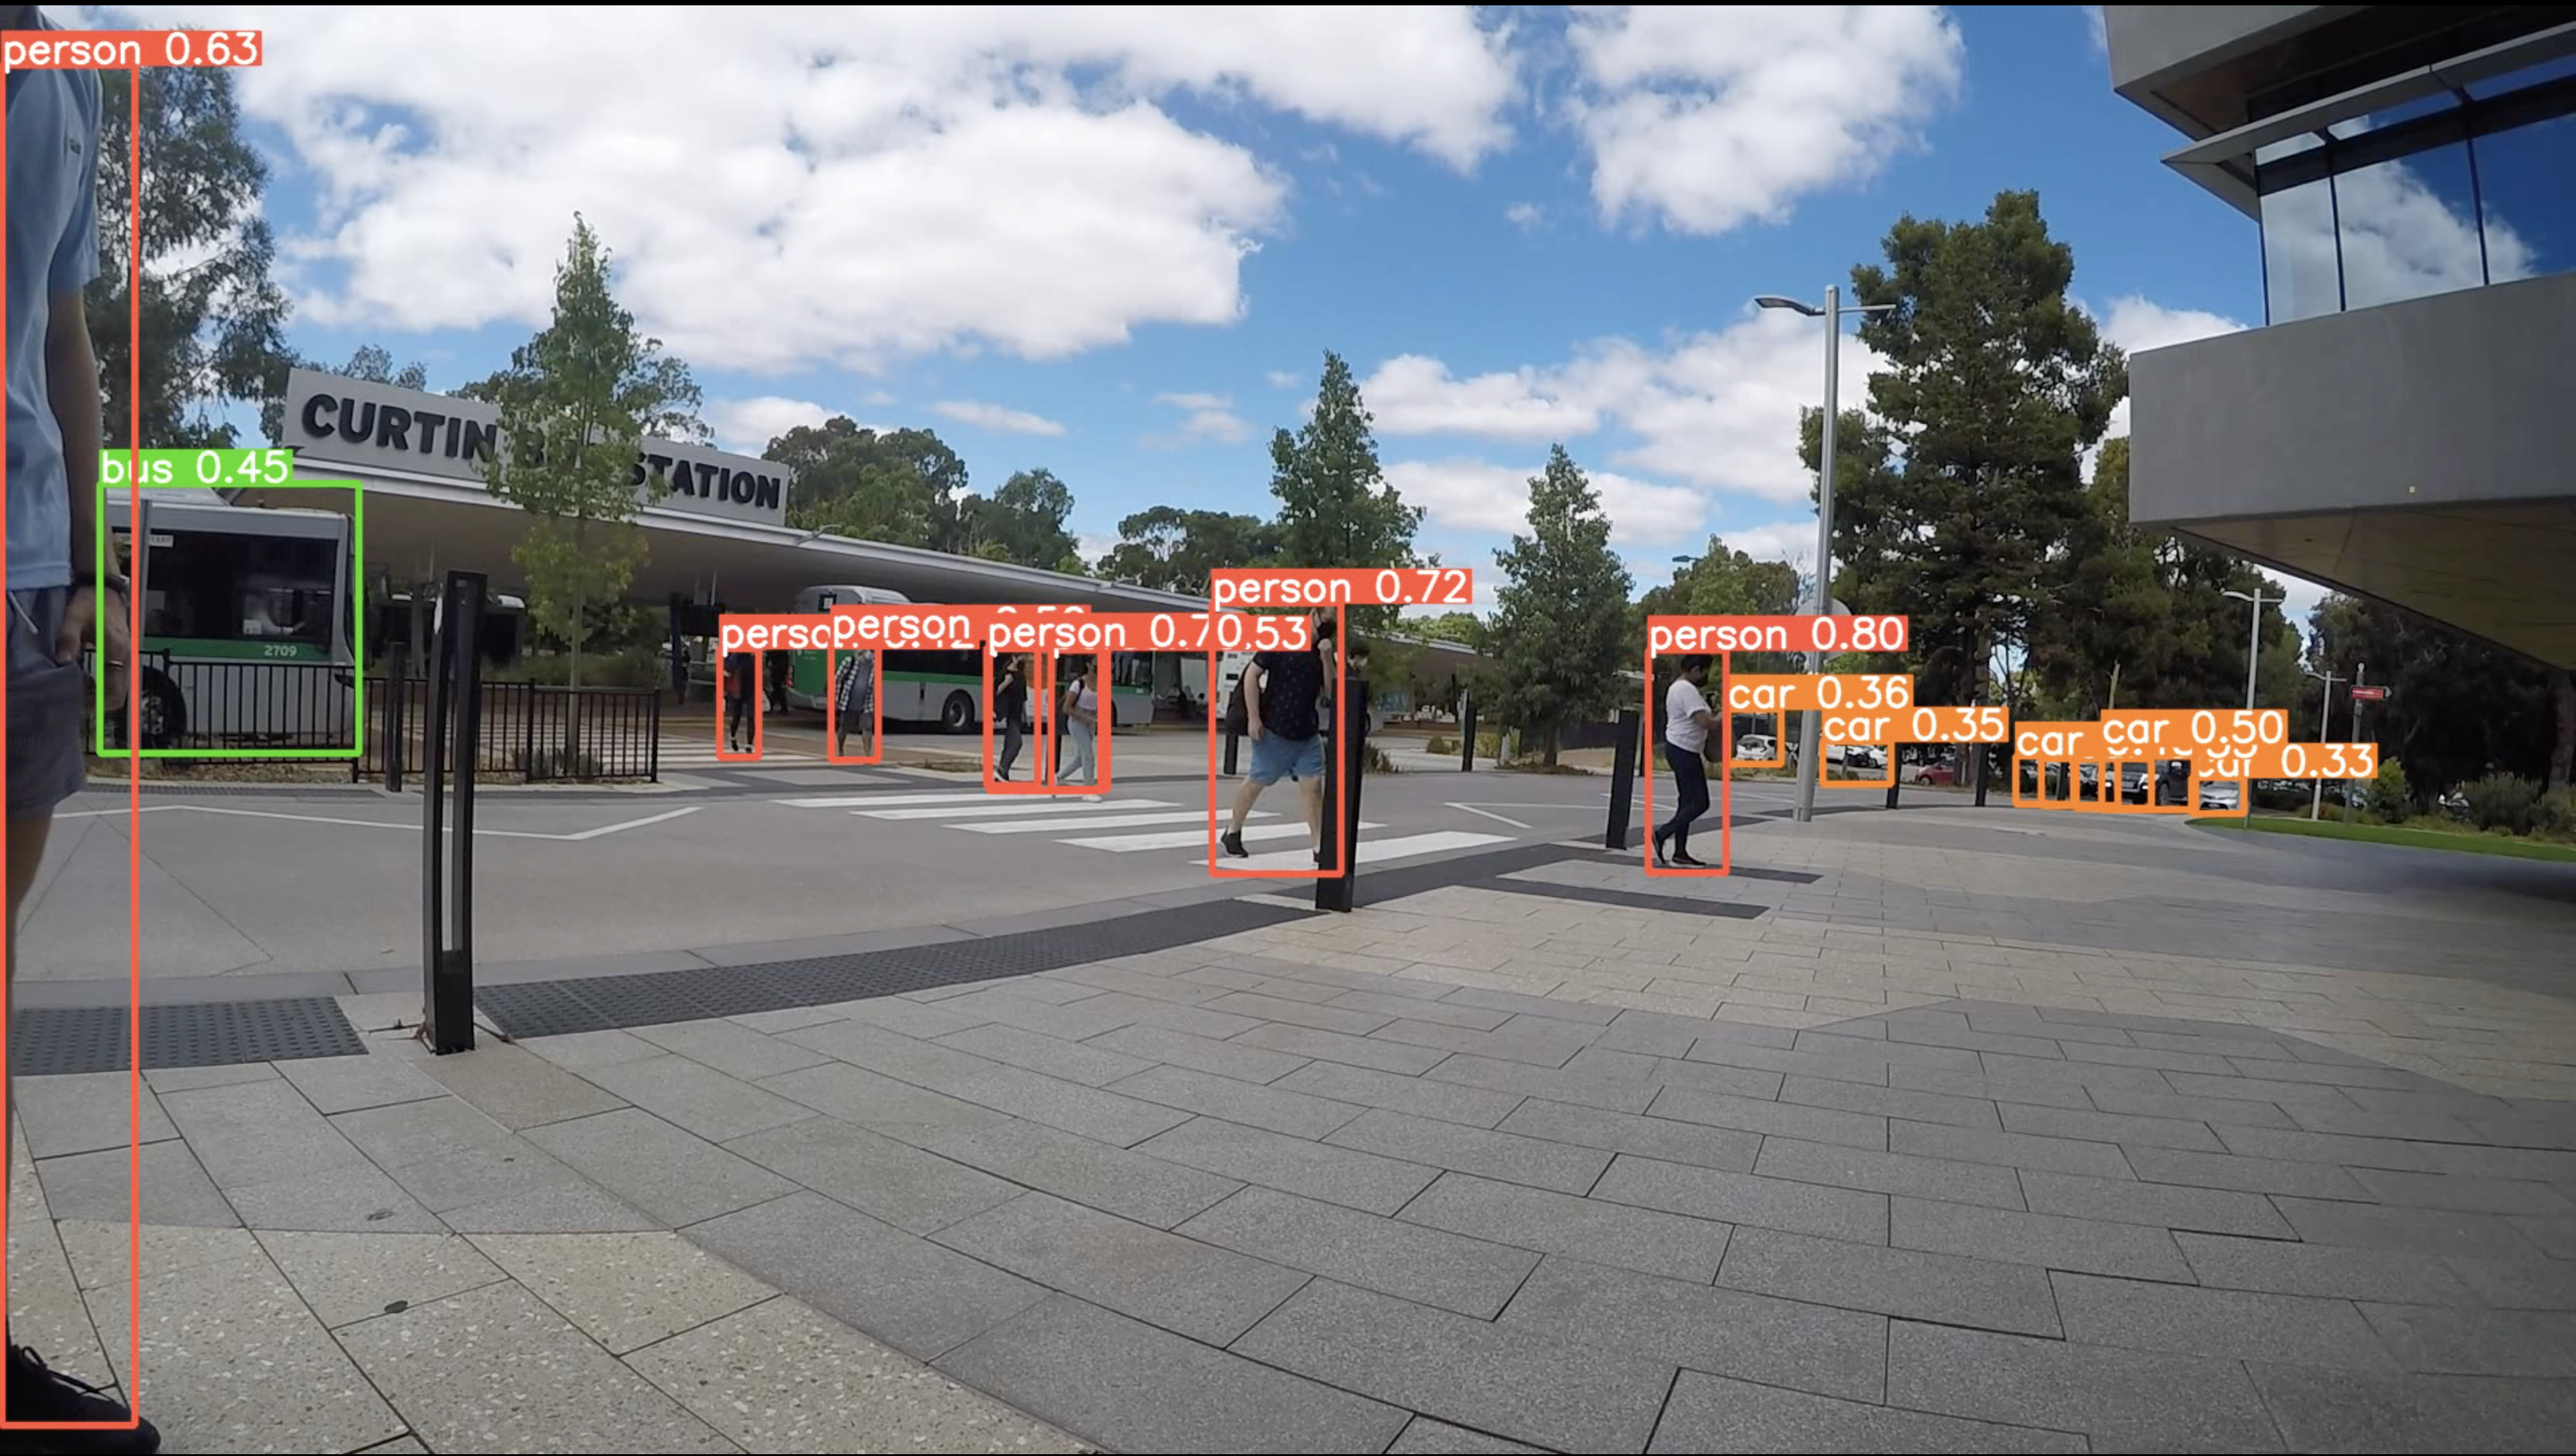
\includegraphics[width=0.65\linewidth]{images/yolov5s.png}
    \caption{YOLOv5s evaluated on the Curtin dataset}
    \label{fig:yolov5s}
\end{figure}

A frame of DeepLabv3 evaluated on the preliminary dataset can be seen in \cref{fig:yolov5s}.
DeepLabv3 identifies pedestrians with a high level of accuracy. However, the vehicles in the
image are not accurately segmented. This is likely due to the lower occurrence of vehicles
in the MS COCO dataset, which was used to train the model.
To repurpose this model for the task of drivable area segmentation,
it would have to be retrained on a labelled driving dataset such as BDD100K or Cityscapes.

\begin{figure}[H]
    \centering
    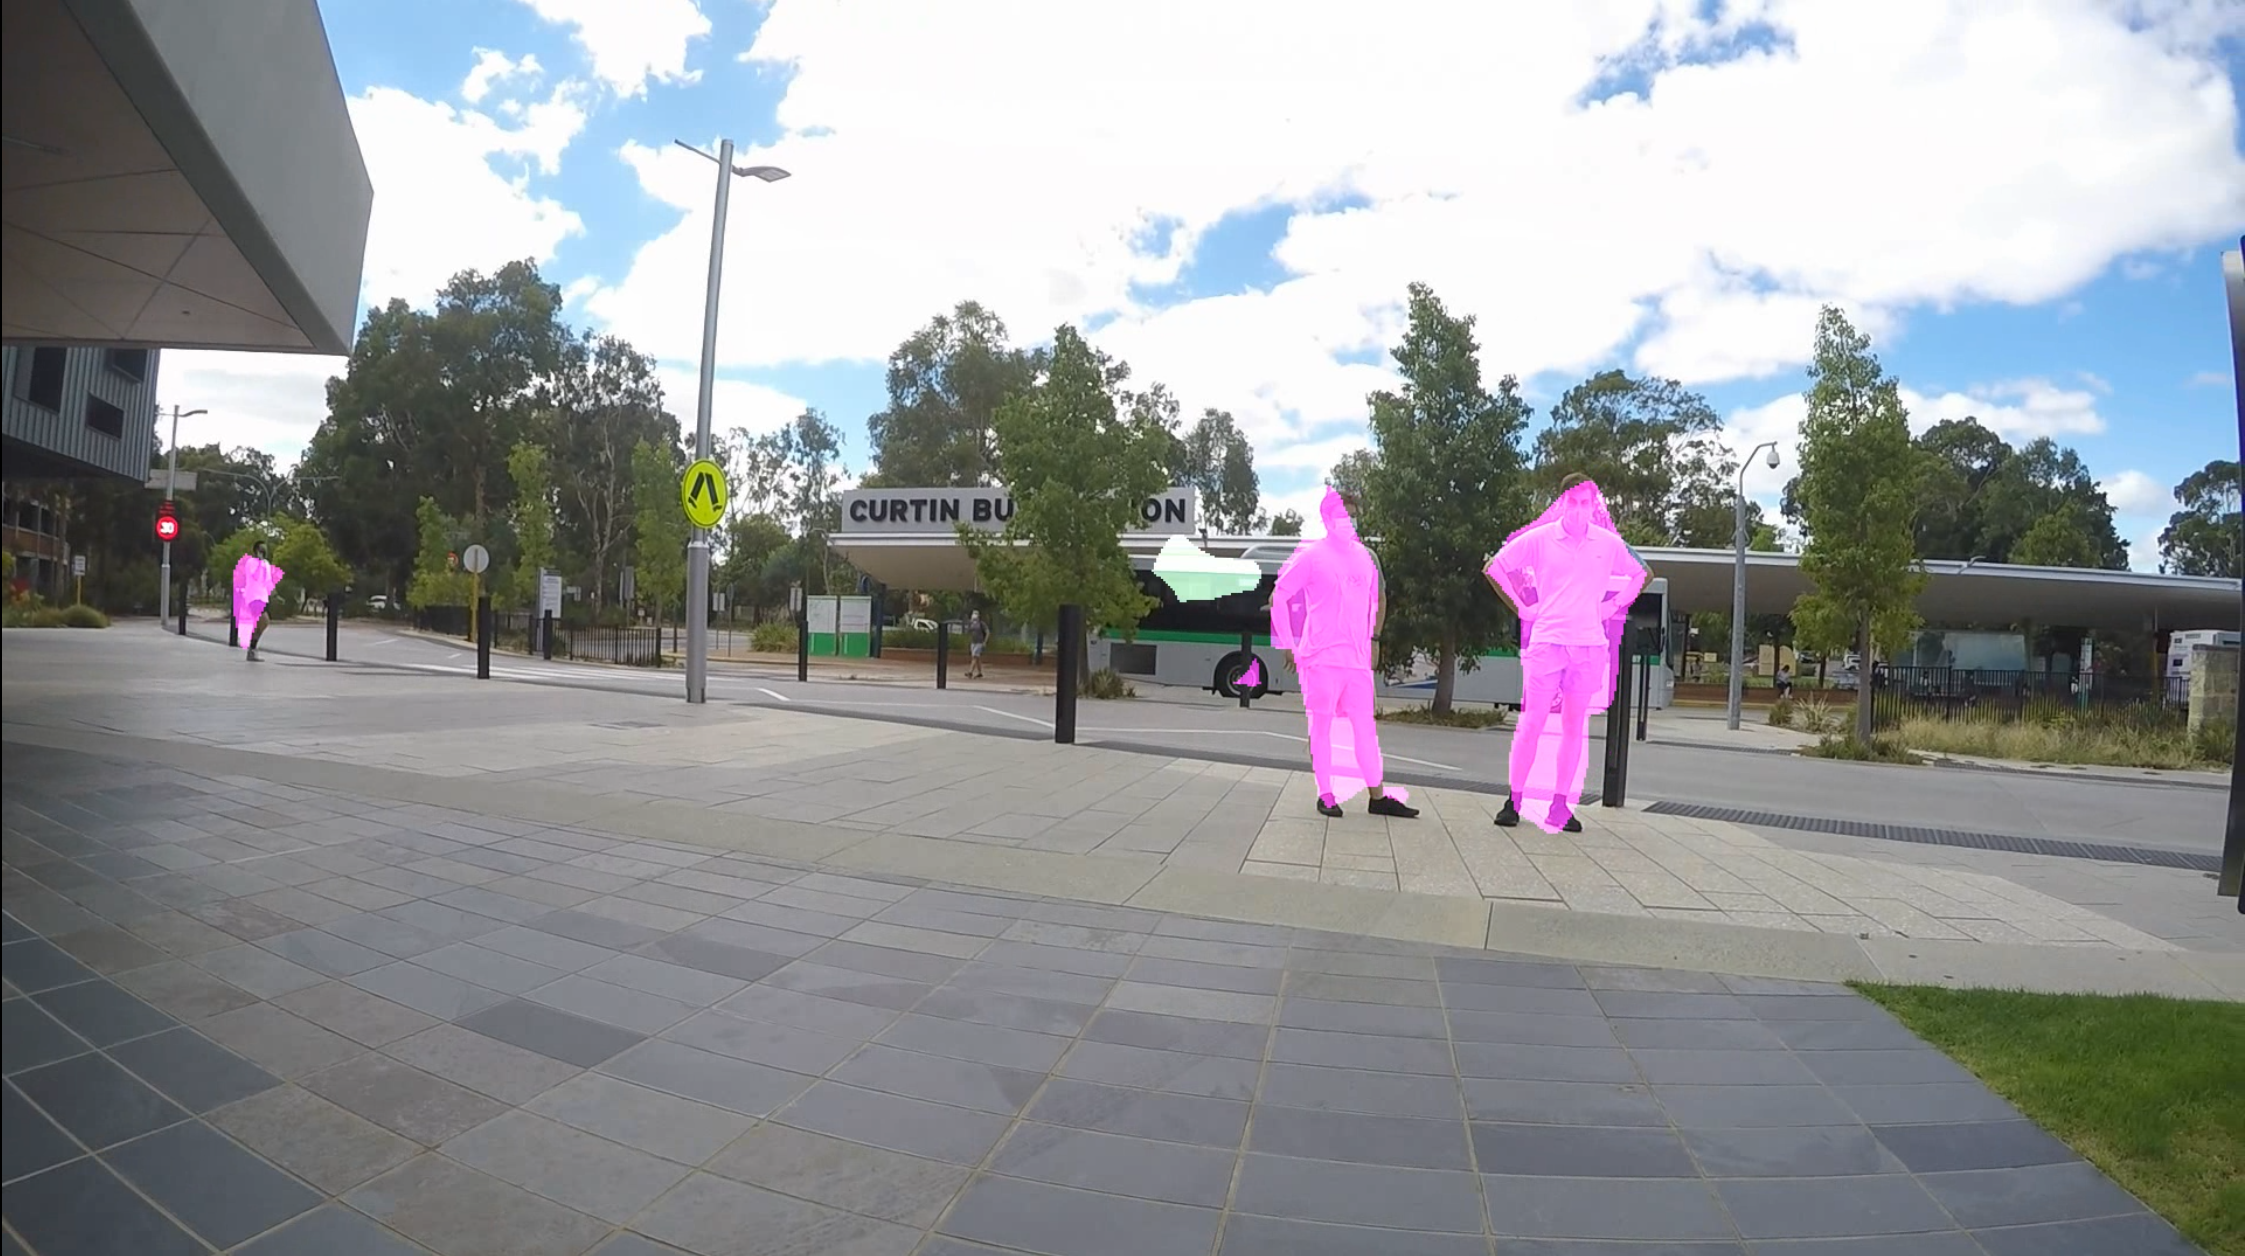
\includegraphics[width=0.65\linewidth]{images/deeplab.png}
    \caption{DeepLabv3 evaluated on the Curtin dataset}
    \label{fig:deeplab}
\end{figure}

An example of Hybridnets drivable area segmentation can be seen in \cref{fig:hybridnets}.
This model accurately detects drivable areas outdoors when a path is uniform, however
has more difficulty identifying a drivable path for non-uniform surfaces such as paved brick.
Hybridnets can also struggle to identify drivable paths indoors in some circumstances.
This is likely due to problems with domain adaptation, as the Hybridnets model was trained on the
BDD100K dataset which primarily consists of bitumen roads.
Hybridnets does not identify drivable area consistently when indoors
but does work well in some cases.

\begin{figure}[H]
    \centering
    \begin{subfigure}{.48\textwidth}
        \centering
        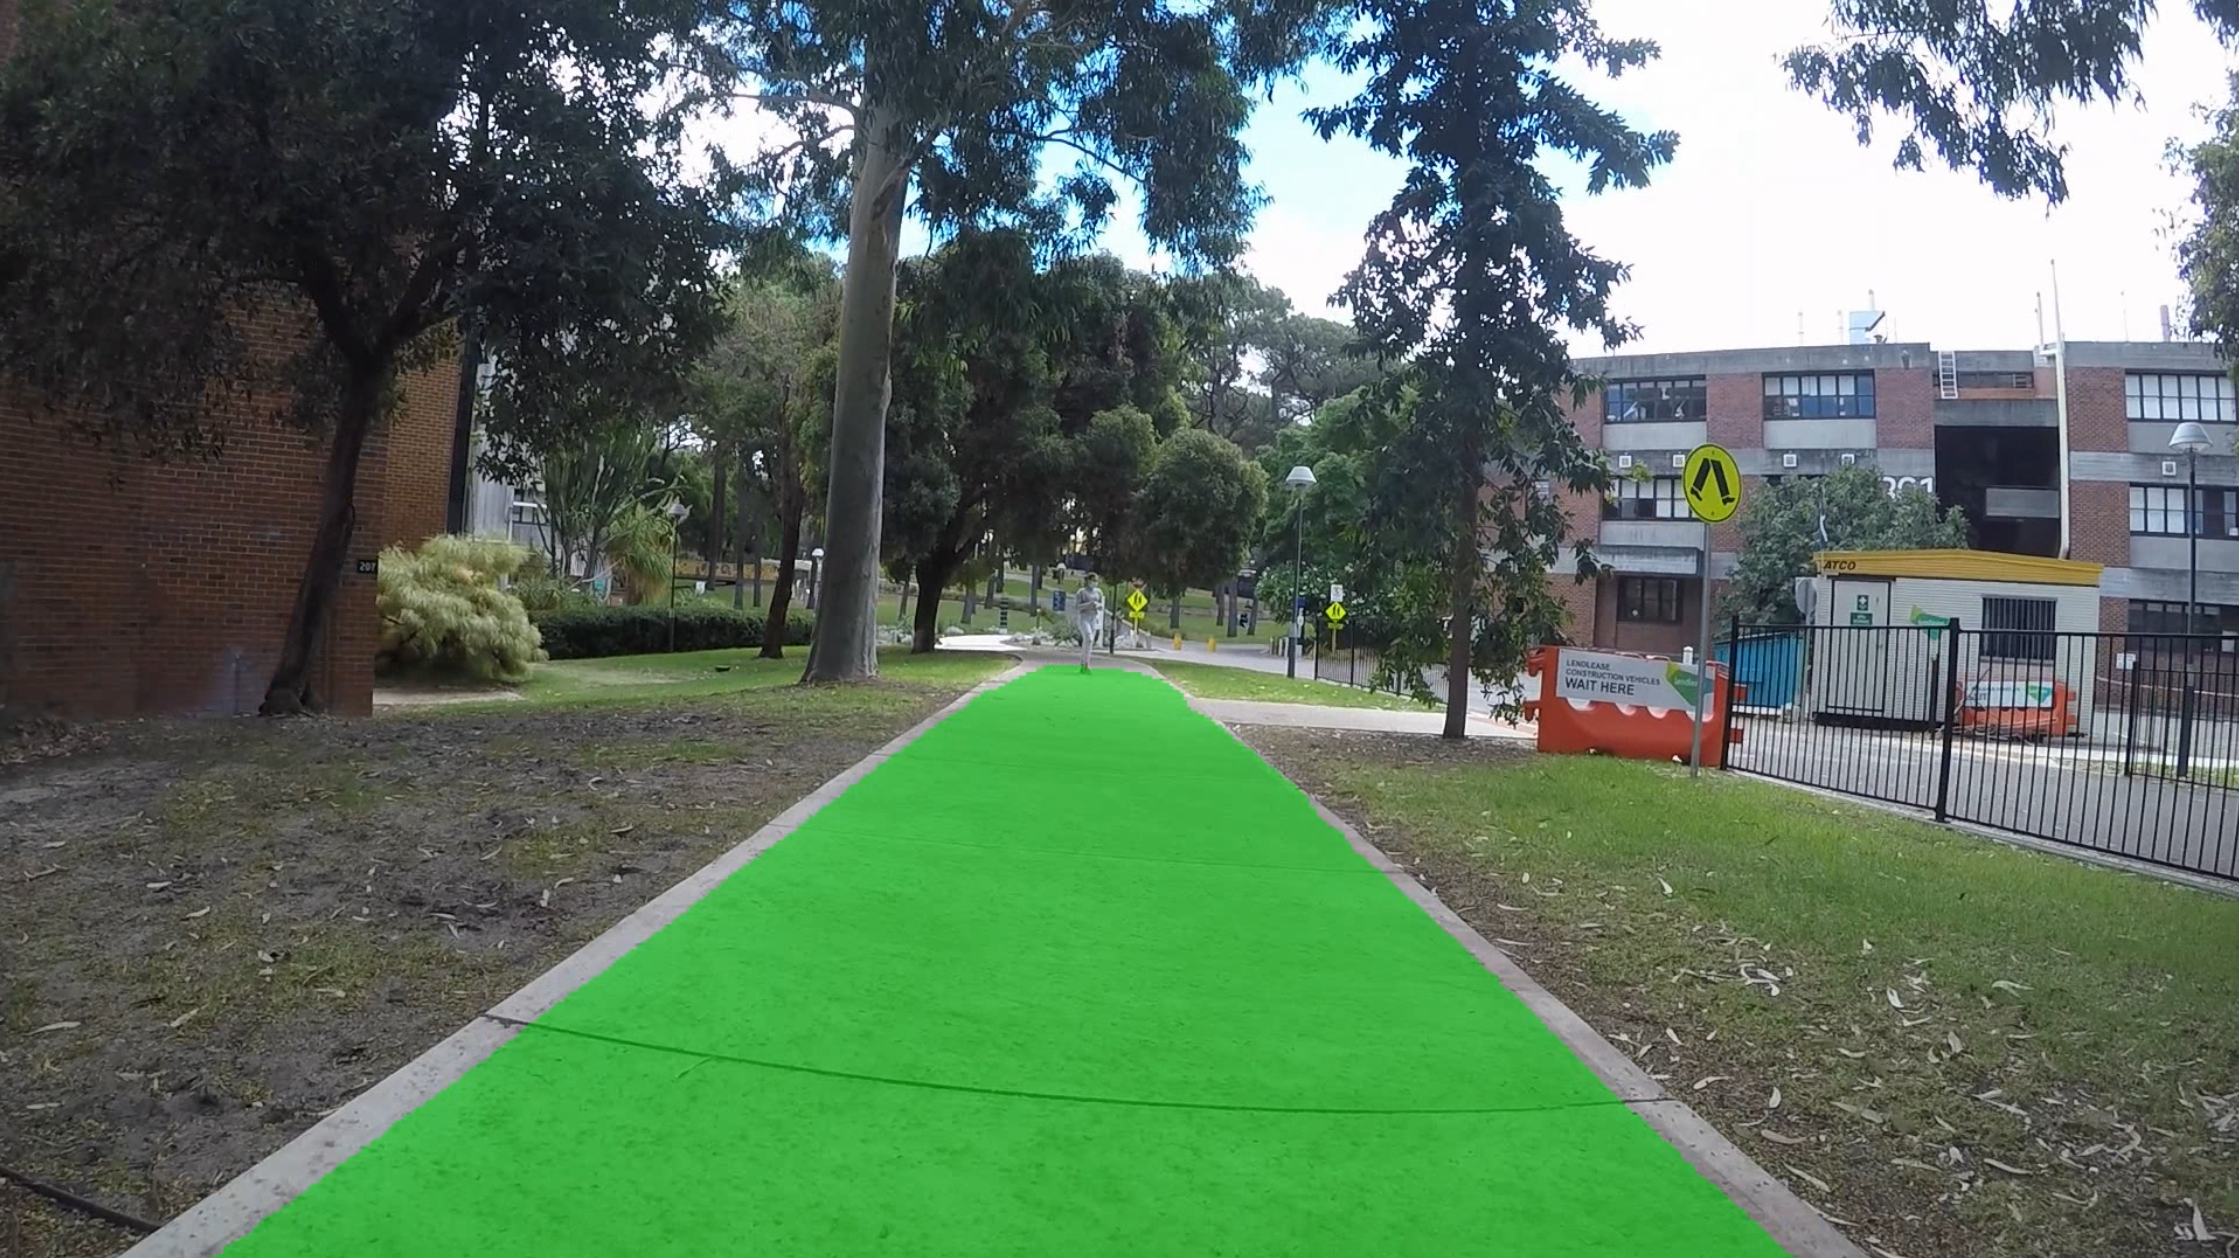
\includegraphics[width=\linewidth]{images/hybridnets_outdoor.png}
        \caption{Outdoors}
    \end{subfigure}
    \quad
    \begin{subfigure}{.47\textwidth}
        \centering
        \includegraphics[width=\linewidth]{images/hybridnets_indoor.png}
        \caption{Indoors}
    \end{subfigure}
    \caption{Hybridnet drivable area segmentation evaluated on the Curtin dataset}
    \label{fig:hybridnets}
\end{figure}

The performance of each model (in frames per second) is given in \cref{table:model_fps}.
This performance was evaluated using a laptop with an RTX 3080 graphics card and AMD Ryzen 9 6900HX processor.
Note that Hybridnets is CPU limited, and could likely be optimized further by modifying postprocessing and video decoding methods.
Additionally,
Hybridnets runs both object detection and image segmentation using the same model.
YOLOv5 runs in real-time on our 24fps dataset, and can likely reach much higher speeds.

\begin{table}[H]
    \centering
    \begin{tabular}{c c c}
    \toprule
    Model Name & FPS & Notes \\
    \midrule
    YOLOv5 & Real-time & (Frame-rate of dataset was 24fps) \\
    DeepLabv3 & 21 &  \\
    Hybridnets & 10 & CPU limited (can likely be optimized) \\
    \bottomrule
    \end{tabular}
    \caption{Performance comparison of ML models}
    \label{table:model_fps}
\end{table}

\subsection{Hybridnets drivable area segmentation}
% do this first
In the last section, it was seen that the Hybridnets model generalised well in most cases,
however struggled with some non-uniform pathways such as paved brick.
The model was originally trained on the BDD100K dataset, which 

\pagebreak
\subsection{Efficiacy of birds-eye view occupancy map transform}
Once the drivable area has been segmented, it is transformed into the XZ plane
as a birds-eye view occupancy map. This is done by processing the 3D point cloud
data from the ZED Mini camera.
Morphological processing is used to improve the density of this occupancy map.
An example of the segmented output alongside the occupancy map can be seen in \cref{fig:occupancy_map_seg},
with the drivable area highlighted in green.
Note that the occupancy map is 15 metres long and 10 metres wide. The location of the ZED Mini camera is depicted
with an `X'; the camera is mounted to the right-hand side of the wheelchair.

\begin{figure}[b]
    % 16:6 width ratio
    % 0.64, 0.24
    \centering
    \begin{subfigure}{.64\textwidth}
        \centering
        \includegraphics[width=\linewidth]{images/segmentation_1.PNG}
    \end{subfigure}
    \quad
    \begin{subfigure}{.24\textwidth}
        \centering
        \includegraphics[width=\linewidth]{images/occupancy_map1.png}
    \end{subfigure}
    \begin{subfigure}{.64\textwidth}
        \centering
        \includegraphics[width=\linewidth]{images/segmentation_2.PNG}
    \end{subfigure}
    \quad
    \begin{subfigure}{.24\textwidth}
        \centering
        \includegraphics[width=\linewidth]{images/occupancy_map2.png}
    \end{subfigure}
    \begin{subfigure}{.64\textwidth}
        \centering
        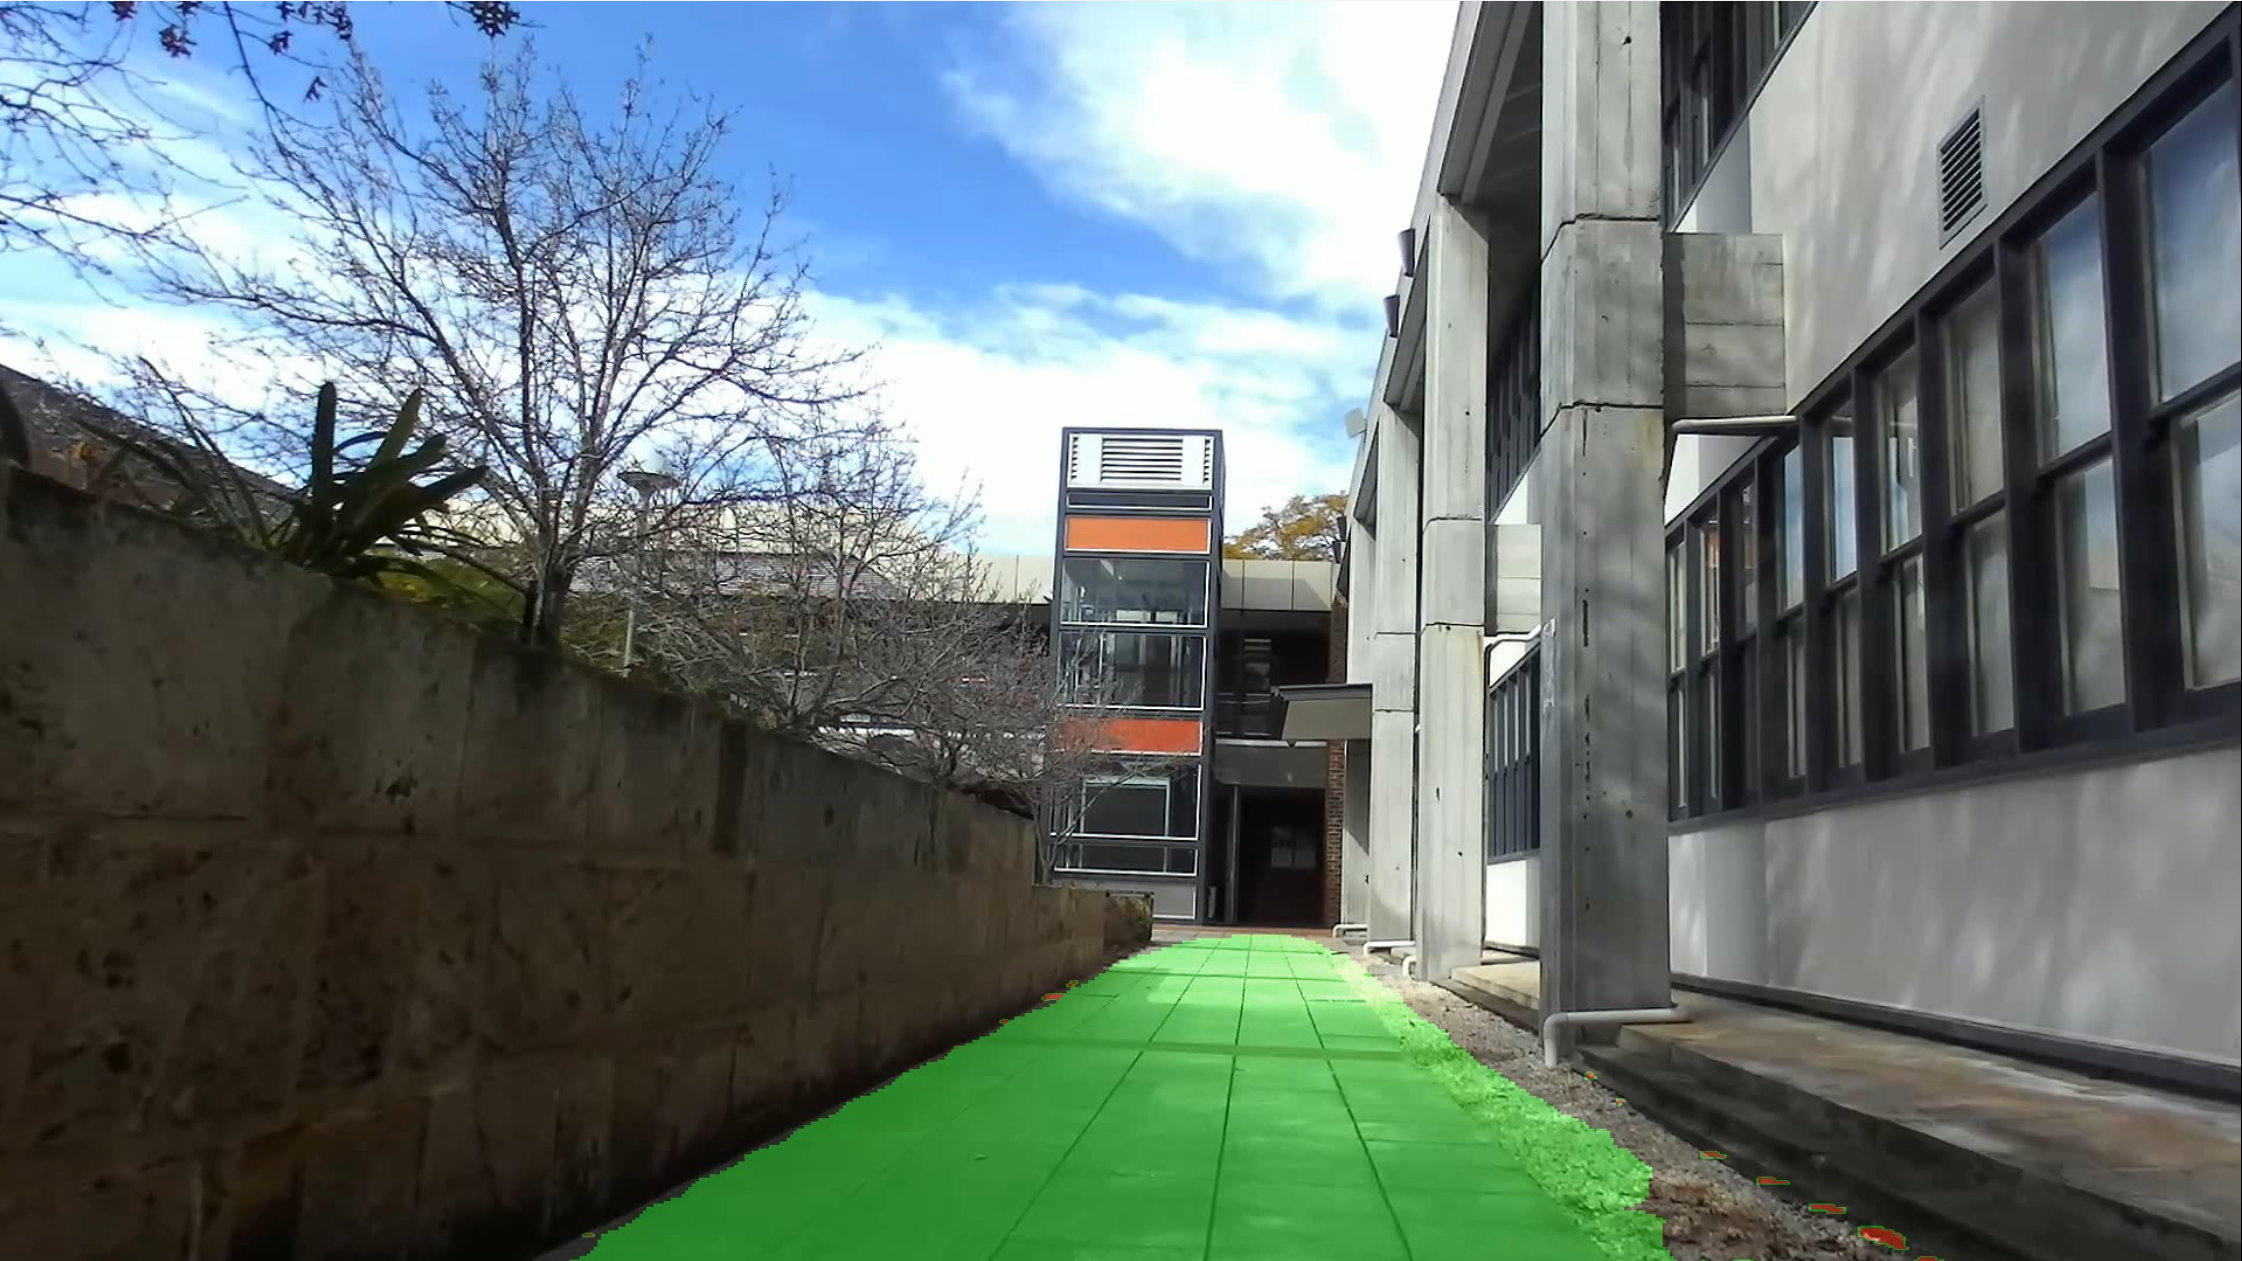
\includegraphics[width=\linewidth]{images/segmentation_3.PNG}
    \end{subfigure}
    \quad
    \begin{subfigure}{.24\textwidth}
        \centering
        \includegraphics[width=\linewidth]{images/occupancy_map3.png}
    \end{subfigure}
    \caption{Segmented image output and corresponding occupancy map for three locations around Curtin university}
    \label{fig:occupancy_map_seg}
\end{figure}

This segmented image to occupancy map transform works well in all observed cases, as long as the Hybridnets model identifies the
drivable area accurately. One improvement that could be made to this implementation is its speed.
The algorithm is bottlenecked by the occupancy map transform code, which takes between \SI{150}{\milli\second}
and \SI{500}{\milli\second} to execute, depending on the size of the drivable area.

Although this approach reliably maps drivable areas to an occupancy grid,
the area directly in front of the wheelchair (approx. \SI{2.6}{\metre}) and behind the wheelchair is unknown due to the FOV of the camera.
Several approaches to rectify this are explored in \cref{sec:future_work}.

A comparison of the occupancy map before and after morphological processing is shown in \cref{fig:morphological_processing}.
Although the occupancy map has a higher resolution before this transformation, the poor density of the map
could make it more difficult to process. The time taken to perform this morphological processing is negligible
when compared to other sections of this code.

\begin{figure}[b]
    % 16:6 width ratio
    % 0.64, 0.24
    \centering
    \begin{subfigure}{.3\textwidth}
        \centering
        \includegraphics[width=\linewidth]{images/occupancy_map1_nomorph.png}
        \caption{Before processing}
    \end{subfigure}
    \quad
    \begin{subfigure}{.3\textwidth}
        \centering
        \includegraphics[width=\linewidth]{images/occupancy_map1.png}
        \caption{After processing}
    \end{subfigure}
    \caption{Comparison of occupancy map before and after morphological processing}
    \label{fig:morphological_processing}
\end{figure}

\subsection{Evaluation of 3D point cloud obstacle detection algorithms}
% sensor tilt, find_floor_plane
% compare performance vs ultra depth mode
Direct processing of the 3D point cloud data was tested to identify environmental obstacles and drivable areas.
One such approach involved using the inbuilt ZED SDK function \texttt{find\_floor\_plane},
which outputs a polygon of the floor plane.
This is shown in \cref{fig:find_floor_plane} and compared alongside the segmentation occupancy map.
This approach is very poor at identifying the floor plane accurately and has large frame-to-frame
variation in its output. The only redeeming factor of this approach is its speed;
as the function is GPU accelerated, this calculation takes approximately \SI{60}{\milli\second}.

\begin{figure}[b]
    % 16:6 width ratio
    % 0.64, 0.24
    \centering
    \begin{subfigure}{.5\textwidth}
        \centering
        \includegraphics[width=\linewidth]{images/find_floor_plane_video.PNG}
        \caption{Video footage}
    \end{subfigure}
    \quad
    \begin{subfigure}{.2\textwidth}
        \centering
        \includegraphics[width=\linewidth]{images/find_floor_plane_seg.PNG}
        \caption{Segmentation occupancy map}
    \end{subfigure}
    \quad
    \begin{subfigure}{.2\textwidth}
        \centering
        \includegraphics[width=\linewidth]{images/find_floor_plane.PNG}
        \caption{Output from \texttt{find\_floor\_plane}}
    \end{subfigure}
    \caption{ZED SDK \texttt{find\_floor\_plane} function compared with segmentation occupancy map}
    \label{fig:find_floor_plane}
\end{figure}

Another approach that was tested was a custom algorithm to process the point cloud data,
detailed in \cref{sec:point_cloud_obstacle_detection}. The results of this algorithm
are shown in three scenarios: one indoor (\cref{fig:pcloud_indoor}) and two outdoor (\cref{fig:pcloud_outdoor_bad} and \cref{fig:pcloud_outdoor_good}).
Note that the drivable area is labelled in green and the environmental obstacles are labelled in red.

\begin{figure}[H]
    % 16:6 width ratio
    % 0.64, 0.24
    \centering
    \begin{subfigure}{.64\textwidth}
        \centering
        \includegraphics[width=\linewidth]{images/pcloud_indoor_video.PNG}
        \caption{Video footage}
    \end{subfigure}
    \quad
    \begin{subfigure}{.24\textwidth}
        \centering
        \includegraphics[width=\linewidth]{images/pcloud_indoor.PNG}
        \caption{Occupancy map}
    \end{subfigure}
    \caption{Point cloud processing result (Indoor)}
    \label{fig:pcloud_indoor}
\end{figure}

\begin{figure}[b]
    % 16:6 width ratio
    % 0.64, 0.24
    \centering
    \begin{subfigure}{.64\textwidth}
        \centering
        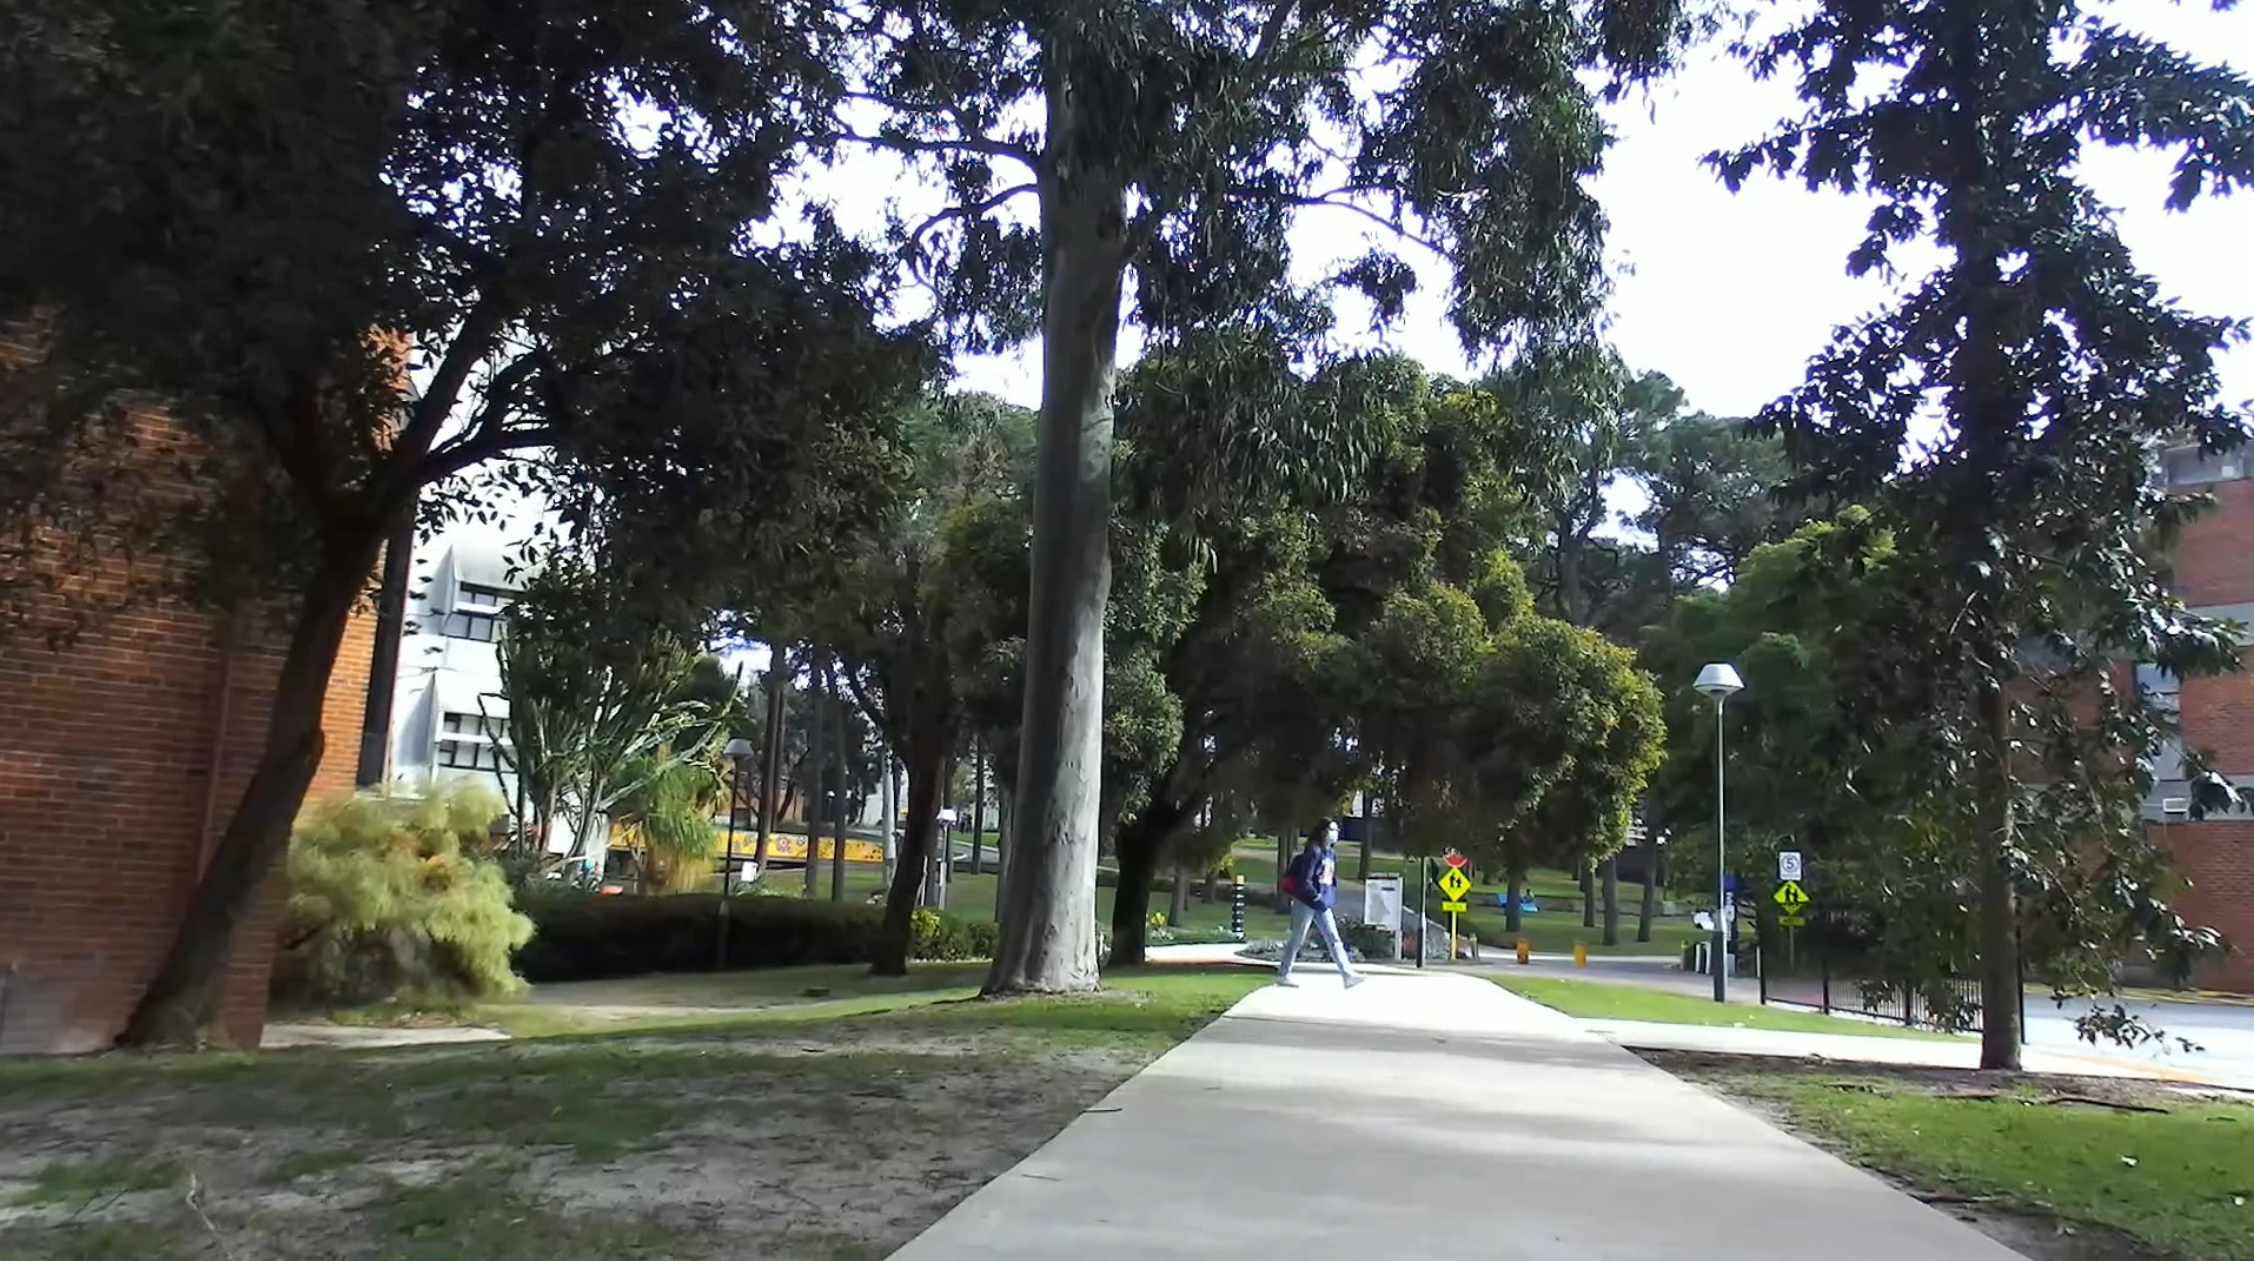
\includegraphics[width=\linewidth]{images/pcloud_outdoor_bad_video.PNG}
        \caption{Video footage}
    \end{subfigure}
    \quad
    \begin{subfigure}{.24\textwidth}
        \centering
        \includegraphics[width=\linewidth]{images/pcloud_outdoor_bad.PNG}
        \caption{Occupancy map}
    \end{subfigure}
    \caption{Point cloud processing result (Outdoor, uniform path)}
    \label{fig:pcloud_outdoor_bad}
\end{figure}

\begin{figure}[b]
    % 16:6 width ratio
    % 0.64, 0.24
    \centering
    \begin{subfigure}{.64\textwidth}
        \centering
        \includegraphics[width=\linewidth]{images/pcloud_outdoor_good_video.PNG}
        \caption{Video footage}
    \end{subfigure}
    \quad
    \begin{subfigure}{.24\textwidth}
        \centering
        \includegraphics[width=\linewidth]{images/pcloud_outdoor_good.PNG}
        \caption{Occupancy map}
    \end{subfigure}
    \caption{Point cloud processing result (Outdoor, wheelchair ramp)}
    \label{fig:pcloud_outdoor_good}
\end{figure}

This algorithm works well in indoor settings (\cref{fig:pcloud_indoor}) at identifying the drivable area
as well as the position of walls and other static objects. Accurate occupancy maps are also generated for
outdoor settings with well-defined boundaries, such as a wheelchair ramp with handrails (\cref{fig:pcloud_outdoor_good}).
However, this algorithm can struggle with open outdoor settings as seen in \cref{fig:pcloud_outdoor_bad}.
Due to the uniformity of the pedestrian path in this image, the ZED Mini is unable to
reliably generate a depth map and 3D point cloud for the path. This leads to the algorithm
mistakenly identifying grassy and uneven terrain as drivable, but not identifying the
path as drivable.

This algorithm is slower than the segmentation approach, with a mean latency of \SI{550}{\milli\second}.
Due to this limitation, it is more suited for identifying non-moving objects such as walls
as opposed to identifying moving objects such as people and vehicles.

The ZED Mini has three depth modes: \texttt{ULTRA}, \texttt{QUALITY}, and \texttt{PERFORMANCE}.
These depth modes trade performance for depth accuracy - a comparison between the occupancy maps
generated by these modes can be seen in \cref{fig:depth_mode_comparison}.
The \texttt{ULTRA} depth mode accurately identifies the back wall as flat.
However, the \texttt{PERFORMANCE} depth mode does not identify the back wall
as flat, and incorrectly classifies an area beyond the wall as drivable.
Due to the high latency of the rest of this algorithm, the difference in speed between these two depth modes is negligible,
and therefore the \texttt{ULTRA} depth mode was selected.

%% can include some ramp comparisons if need be, but probably not

\begin{figure}[b]
    % 16:6 width ratio
    % 0.64, 0.24
    \centering
    \begin{subfigure}{.5\textwidth}
        \centering
        \includegraphics[width=\linewidth]{images/pcloud_indoor_comparison.PNG}
        \caption{Video footage}
    \end{subfigure}
    \quad
    \begin{subfigure}{.2\textwidth}
        \centering
        \includegraphics[width=\linewidth]{images/pcloud_indoor_performance.PNG}
        \caption{Performance depth mode}
    \end{subfigure}
    \begin{subfigure}{.2\textwidth}
        \centering
        \includegraphics[width=\linewidth]{images/pcloud_indoor_ultra.PNG}
        \caption{Ultra depth mode}
    \end{subfigure}
    \caption{Comparison of ZED Mini depth modes}
    \label{fig:depth_mode_comparison}
\end{figure}

\subsection{Evaluation of assistive control algorithm}
VFH+ was implemented as a proof-of-concept assistive control algorithm.
This algorithm blends the user's target direction with the occupancy map
to determine a safe steering direction.

\Cref{fig:vfh_implementation} shows the VFH+ algorithm detecting an obstacle in front of
the wheelchair and steering left to avoid this obstacle. This
%demonstrates that  VFH+ works reliably as an assistive control algorithm and
showcases the end-to-end navigation assistance pipeline,
from environmental obstacle detection to
avoidance of that obstacle using VFH+.

The VFH+ algorithm takes
\SI{240}{\milli\second} to determine the steering direction, which increases to
\SI{430}{\milli\second} when called from Python due to the overhead of the MATLAB Engine API.
This latency could be a concern for a complete semi-autonomous wheelchair implementation;
however, this algorithm is a proof of concept, and latency was not a concern during implementation.
Additionally, VFH+ only adjusts the direction of the wheelchair and not the wheelchair's speed,
making it unsuitable as a final assistive control algorithm.

Due to the FOV of the camera, obstacles directly to the left or right of the wheelchair are not added
to the occupancy map. \Cref{fig:vfh_mistake} demonstrates a scenario where this can
become an issue. VFH+ mistakenly steers to the left to avoid the narrow hallway walls,
which would cause a crash with the walls directly to the left of the wheelchair.
This occurs because these walls are not in the occupancy map, and so the VFH+ algorithm
assumes that there is free space in this area.
Several approaches that could improve the occupancy map and rectify this issue
are suggested in \cref{sec:future_work}.

\begin{figure}[b]
    % 16:6 width ratio
    % 0.64, 0.24
    \centering
    \begin{subfigure}{.6\textwidth}
        \centering
        \includegraphics[width=\linewidth]{images/vfh_example_video.PNG}
        \caption{Video footage}
    \end{subfigure}
    \quad
    \begin{subfigure}{.3\textwidth}
        \centering
        \includegraphics[width=\linewidth]{images/vfh_example_map.PNG}
        \caption{Occupancy map}
    \end{subfigure}
    \begin{subfigure}{.45\textwidth}
        \centering
        \includegraphics[width=\linewidth]{images/vfh_example_lidar.PNG}
        \caption{Binary occupancy grid and LIDAR scan of obstacles}
    \end{subfigure}
    \quad
    \begin{subfigure}{.45\textwidth}
        \centering
        \includegraphics[width=\linewidth]{images/vfh_example_hist.PNG}
        \caption{Polar histogram of obstacles with target and steering directions}
    \end{subfigure}
    \caption{VFH+ changing direction to avoid an obstacle}
    \label{fig:vfh_implementation}
\end{figure}

\begin{figure}[b]
    % 16:6 width ratio
    % 0.64, 0.24
    \centering
    \begin{subfigure}{.6\textwidth}
        \centering
        \includegraphics[width=\linewidth]{images/vfh_fov_video.PNG}
        \caption{Video footage}
    \end{subfigure}
    \quad
    \begin{subfigure}{.3\textwidth}
        \centering
        \includegraphics[width=\linewidth]{images/vfh_fov_map.PNG}
        \caption{Occupancy map}
    \end{subfigure}
    \begin{subfigure}{.45\textwidth}
        \centering
        \includegraphics[width=\linewidth]{images/vfh_fov_lidar.PNG}
        \caption{Binary occupancy grid and LIDAR scan of obstacles}
    \end{subfigure}
    \quad
    \begin{subfigure}{.45\textwidth}
        \centering
        \includegraphics[width=\linewidth]{images/vfh_fov_hist.PNG}
        \caption{Polar histogram of obstacles with target and steering directions}
    \end{subfigure}
    \caption{VFH+ mistakenly changing direction due to low sensor FOV}
    \label{fig:vfh_mistake}
\end{figure}

% include speed, turning behind

\subsection{Evaluation of pose estimation APIs}
% positional tracking API

\cleardoublepage

\section{CONCLUSIONS}
\cleardoublepage

\section{FUTURE WORK}
\input{chapters/future_work.tex}
\cleardoublepage

\printbibliography[title={REFERENCES},heading=bibnumbered]
\cleardoublepage

\appendix
\section*{APPENDIX A - Thesis Completion Form}
\addcontentsline{toc}{section}{APPENDIX A - Thesis Completion Form}
\cleardoublepage
\includepdf{ThesisCompletionForm.pdf}

\cleardoublepage
\section*{APPENDIX B - Datasets and code}
\addcontentsline{toc}{section}{APPENDIX B - Datasets and code}
%\addcontentsline{toc}{section}{APPENDIX B - Thesis Planning}
%Time should be allocated to thesis writing and review as well as technical progress.
%A Gantt chart displaying the expected progress over the course of the two semesters
%is shown in \cref{fig:gantt_chart}. Note that a significant portion of time at the beginning was allocated
%to initial research and project scope. Due to the large number of students working on this team,
%a clear project scope was important so that students did not unnecessarily duplicate work.

%\begin{figure}[H]
%    \centering
%    \includegraphics[width=\linewidth]{images/gantt_chart.png}
%    \caption{Gantt chart of thesis progress}
%    \label{fig:gantt_chart}
%\end{figure}
% TODO update Gantt chart

All supplementary material for this thesis has been submitted on a USB thumbdrive.
Some supplementary material has also been uploaded to the 'Curtin X Glide (Smart Wheelchair)' Teams channel so that it can be used by future thesis students
working on this project. Links to each of these files are provided.
\begin{itemize}
    \item The preliminary Curtin University video-only driving dataset is hosted on \href{https://curtin.sharepoint.com/:v:/r/sites/CurtinXGlide/Shared%20Documents/Navigation%20and%20Object%20Detection/GoPro%20Dataset.mp4?csf=1&web=1&e=seLdRb}{\underline{Teams}}.
    \item The ZED Mini RGB-D Curtin University driving dataset is also hosted on \href{https://curtin.sharepoint.com/:f:/r/sites/CurtinXGlide/Shared%20Documents/Navigation%20and%20Object%20Detection/ZED?csf=1&web=1&e=tTau9D}{\underline{Teams}}.
    \item The BDD100K and Cityscapes datasets used to train and evaluate the segmentation model have been uploaded to \href{https://curtin.sharepoint.com/:f:/r/sites/CurtinXGlide/Shared%20Documents/Navigation%20and%20Object%20Detection/External%20Datasets?csf=1&web=1&e=qjWuoP}{\underline{Teams}}.
\end{itemize}

Some material specific to this thesis has also been uploaded to the \href{https://curtin.sharepoint.com/:f:/r/sites/CurtinXGlide/Shared%20Documents/Navigation%20and%20Object%20Detection/Jakob?csf=1&web=1&e=KUuiUt}{\underline{Teams channel}}.
This material includes:
\begin{itemize}
    \item \textbf{datasets/zed/labelled}: Drivable area annotations for a portion of the Curtin RGB-D driving dataset. Refer to appendix D for further information.
    \item \textbf{datasets/zed/video}: The Curtin RGB-D driving dataset converted into the avi video format, for use with devices that may not have the ZED SDK installed.
    \item \textbf{models}: Model weights for trained ML models, saved at each training epoch.
    \item \textbf{results}: Video results for segmentation, obstacle detection, and assistive control algorithms (tested on the Curtin RGB-D driving dataset).
\end{itemize}

All code used in this thesis can be found on \href{https://github.com/JakobWyatt/smart-wheelchair}{\underline{Github}}.
This repository contains:
\begin{itemize}
    \item \textbf{code}: Python and MATLAB code used to implement various algorithms.
    \item \textbf{colab}: Colab notebooks used to train the segmentation model.
    \item \textbf{environments}: Conda environments used to manage dependencies.
    \item \textbf{models}: 3D models for the ZED mount (Inventor, Fusion, STL).
    \item \textbf{repositories}: Git submodules and sample code.
\end{itemize}
This repository also contains the latex source code used to format this document.


\end{document}
